\documentclass{ieeeaccess}

\usepackage{cite}
\usepackage{amsmath,amssymb,amsfonts}
\usepackage{algorithmic}
\usepackage{graphicx}
\usepackage{textcomp}

\usepackage{bm}
\makeatletter
\AtBeginDocument{\DeclareMathVersion{bold}
\SetSymbolFont{operators}{bold}{T1}{times}{b}{n}
\SetSymbolFont{NewLetters}{bold}{T1}{times}{b}{it}
\SetMathAlphabet{\mathrm}{bold}{T1}{times}{b}{n}
\SetMathAlphabet{\mathit}{bold}{T1}{times}{b}{it}
\SetMathAlphabet{\mathbf}{bold}{T1}{times}{b}{n}
\SetMathAlphabet{\mathtt}{bold}{OT1}{pcr}{b}{n}
\SetSymbolFont{symbols}{bold}{OMS}{cmsy}{b}{n}
\renewcommand\boldmath{\@nomath\boldmath\mathversion{bold}}}
\makeatother

\def\BibTeX{{\rm B\kern-.05em{\sc i\kern-.025em b}\kern-.08em
    T\kern-.1667em\lower.7ex\hbox{E}\kern-.125emX}}

\usepackage{algorithm}
\usepackage{booktabs}
\usepackage{microtype}
\usepackage{needspace}
\usepackage{url}
\def\UrlBreaks{\do\/\do\-\do\a\do\b\do\c\do\d\do\e\do\f\do\0\do\1\do\2\do\3\do\4\do\5\do\6\do\7\do\8\do\9}
\usepackage{tabularx}
\usepackage{multirow}
\usepackage[
    hidelinks,
    bookmarks=false,
    pdftitle={Is Sub-Byte Weight Quantization Worth It on Microcontrollers? Measured Sensitivity, Allocation Algorithms, and a Hardware Cost Model},
    pdfauthor={Dhruv Narayan Bajaj}
]{hyperref}

% Enforce Roman numerals for tables (D7 / access.tex)
\renewcommand{\thetable}{\Roman{table}}

% Auto-generated empirical macros for Sub-Byte MCU Paper
% Traceable directly to multi-seed results store
\newcommand{\MacroBaselineParams}{502{,}222}
\newcommand{\MacroSeparableCNNTotalParams}{502{,}222}
\newcommand{\MacroSeparableCNNWeights}{496{,}224}
\newcommand{\MacroResNetEightTotalParams}{78{,}042}
\newcommand{\MacroResNetEightWeights}{77{,}360}
\newcommand{\MacroBaselineFPBytes}{1{,}986.2}
\newcommand{\MacroMaxPossibleINTEightKiB}{496.5}
\newcommand{\MacroPeakActivationKB}{45}
\newcommand{\MacroRandomAllocCount}{200}
\newcommand{\MacroHSSThreshold}{0.40}
\newcommand{\MacroSearchLayersMax}{20}
\newcommand{\MacroSearchBitwidthsCount}{7}
\newcommand{\MacroKnapsackSolveTimeMs}{3.11}
\newcommand{\MacroCIFARTenResNetFPAcc}{83.98}
\newcommand{\MacroCIFARTenSeparableCNNFPAcc}{87.53}
\newcommand{\MacroFMNISTFPAcc}{91.80}
\newcommand{\MacroSpeechFPAcc}{91.73}
\newcommand{\MacroHARFPAcc}{93.73}
\newcommand{\MacroCIFARTenResNetINTEightAcc}{84.17}
\newcommand{\MacroCIFARTenSeparableCNNINTEightAcc}{86.11}
\newcommand{\MacroFMNISTINTEightAcc}{91.30}
\newcommand{\MacroSpeechINTEightAcc}{92.20}
\newcommand{\MacroHARINTEightAcc}{93.36}
\newcommand{\MacroDeployableSpeedup}{1.35}
\newcommand{\MacroBreakEvenPenalty}{1.35}
\newcommand{\MacroBreakEvenPenaltySIMD}{1.00}
\newcommand{\MacroDeployableAccDelta}{0.22}
\newcommand{\MacroFTEpochs}{5}
\newcommand{\MacroFTGainCompensate}{0.5}
\newcommand{\MacroVarianceDominancePct}{92.7}
\newcommand{\MacroAdditivityRho}{0.941}
\newcommand{\MacroAdditivityMAE}{16.97}
\newcommand{\MacroAdditivityMAERaw}{21.29}
\newcommand{\MacroAdditivityRhoRaw}{0.943}
\newcommand{\MacroResNetRho}{-0.055}
\newcommand{\MacroSpeechRho}{-0.539}
\newcommand{\MacroSeparableCNNRho}{0.286}
\newcommand{\MacroPartialRho}{0.240}
\newcommand{\MacroResNetPartialRho}{0.042}
\newcommand{\MacroSpeechPartialRho}{-0.412}
\newcommand{\MacroUnpackThreeBitPenalty}{2.12}
\newcommand{\MacroSubByteUnpackPenalty}{3.41}
\newcommand{\MacroUnpackFourBitPenalty}{1.16}
\newcommand{\MacroUnpackTwoBitPenalty}{0.98}
\newcommand{\MacroUnpackFourBitSIMD}{1.56}
\newcommand{\MacroUnpackTwoBitSIMD}{1.33}
\newcommand{\MacroCMSISBaselineCyclesPerMAC}{3.38}
\newcommand{\MacroBaselinePenalty}{1.00}
\newcommand{\MacroMaxDeployableSpeedup}{1.55}
\newcommand{\MacroFixedRhoTarget}{0.80}
\newcommand{\MacroFixedMAETarget}{1.0}
\newcommand{\MacroPairedN}{5}
\newcommand{\MacroCyclesFourBitSIMD}{5.28}
\newcommand{\MacroCyclesFourBitScalar}{4.52}
\newcommand{\MacroCyclesTwoBitSIMD}{4.51}
\newcommand{\MacroCyclesTwoBitScalar}{3.82}
\newcommand{\MacroCyclesThreeBit}{12.23}
\newcommand{\MacroCyclesFiveBit}{13.23}
\newcommand{\MacroCyclesSevenBit}{13.24}
\newcommand{\MacroPenaltySevenBit}{3.41}
\newcommand{\MacroCrossoverThresholdBudget}{40}
\newcommand{\MacroCrossoverThresholdBits}{3.2}
\newcommand{\MacroTotalVarianceSumPct}{100.0}
\newcommand{\MacroCoreFrequencyMHz}{180}
\newcommand{\MacroTargetArch}{ARM Cortex-M4}
\newcommand{\MacroTargetCore}{Cortex-M4}
\newcommand{\MacroBootDPHAWQMeanFT}{0.55}
\newcommand{\MacroBootDPHAWQMedianFT}{0.37}
\newcommand{\MacroBootDPHAWQCILowFT}{-0.25}
\newcommand{\MacroBootDPHAWQCIHighFT}{0.95}
\newcommand{\MacroBootDPHAWQWilcoxonFT}{0.0}
\newcommand{\MacroBootDPHAWQWilcoxonPFT}{0.0625}
\newcommand{\MacroBootDPHAWQMeanCollapse}{0.47}
\newcommand{\MacroBootDPHAWQMedianCollapse}{0.20}
\newcommand{\MacroBootDPHAWQCILowCollapse}{-0.10}
\newcommand{\MacroBootDPHAWQCIHighCollapse}{0.74}
\newcommand{\MacroBootDPHAWQWilcoxonCollapse}{0.0}
\newcommand{\MacroBootDPHAWQWilcoxonPCollapse}{0.0625}
\newcommand{\MacroBootDPHAWQMeanPlateau}{0.62}
\newcommand{\MacroBootDPHAWQMedianPlateau}{0.47}
\newcommand{\MacroBootDPHAWQCILowPlateau}{0.43}
\newcommand{\MacroBootDPHAWQCIHighPlateau}{0.89}
\newcommand{\MacroBootDPHAWQWilcoxonPlateau}{0.0}
\newcommand{\MacroBootDPHAWQWilcoxonPPlateau}{0.1250}
\newcommand{\MacroBootDPGreedyMeanFT}{0.02}
\newcommand{\MacroBootDPGreedyMedianFT}{0.01}
\newcommand{\MacroBootDPGreedyCILowFT}{-0.10}
\newcommand{\MacroBootDPGreedyCIHighFT}{0.15}
\newcommand{\MacroBootDPGreedyWilcoxonFT}{1.0}
\newcommand{\MacroBootDPGreedyWilcoxonPFT}{0.1250}
\newcommand{\MacroSeedLevelPositiveFiftyCount}{21}
\newcommand{\MacroSeedLevelPositiveFiftyTotal}{25}
\newcommand{\MacroSeedLevelPositiveFiftyP}{0.0009}
\newcommand{\MacroSeedLevelPositiveSeventyFiveCount}{19}
\newcommand{\MacroSeedLevelPositiveSeventyFiveTotal}{25}
\newcommand{\MacroSeedLevelPositiveSeventyFiveP}{0.0146}
\newcommand{\MacroHARDeltasTwentyFive}{0.01}
\newcommand{\MacroHARDeltasThirtyFive}{0.39}
\newcommand{\MacroHARDeltasFifty}{-0.08}
\newcommand{\MacroHARDeltasSeventyFive}{0.14}
\newcommand{\MacroHARDeltasMean}{0.11}
\newcommand{\MacroFloorDeltaSepCNN}{-0.07}
\newcommand{\MacroFloorDeltaResNet}{0.07}
\newcommand{\MacroFloorDeltaFMNIST}{0.05}
\newcommand{\MacroFloorDeltaSpeech}{0.01}
\newcommand{\MacroFloorDeltaHAR}{0.01}
\newcommand{\MacroDPHARDeficitMean}{0.11}
\newcommand{\MacroDPHARDeficitMeanClean}{0.11}
\newcommand{\MacroSpeechGainFifty}{2.39}
\newcommand{\MacroSpeechFiftyDP}{91.69}
\newcommand{\MacroSpeechFiftyHAWQ}{89.30}
\newcommand{\MacroSeparableCNNThirtyFiveGain}{2.47}
\newcommand{\MacroDPFMNISTThirtyFiveDeficit}{0.19}
\newcommand{\MacroDPFMNISTFiftyDeficitMean}{0.11}
\newcommand{\MacroFMNISTFiftyUniformWFourAdv}{0.15}
\newcommand{\MacroDPUniformWFourMinFifty}{-0.24}
\newcommand{\MacroDPUniformWFourMaxFifty}{+0.28}
\newcommand{\MacroDPUniformWFourMinSeventyFive}{-0.11}
\newcommand{\MacroDPUniformWFourMaxSeventyFive}{+0.31}
\newcommand{\MacroDPUniformWFourMinCombined}{-0.24}
\newcommand{\MacroDPUniformWFourMaxCombined}{+0.31}
\newcommand{\MacroDPUniformWFourAbsMaxCombined}{0.31}
\newcommand{\MacroPTQMedianDeltaThirtyFive}{18.91}
\newcommand{\MacroPTQMeanDeltaThirtyFive}{26.49}
\newcommand{\MacroPTQMeanDeltaFifty}{5.36}
\newcommand{\MacroPTQMeanDeltaSeventyFive}{0.52}
\newcommand{\MacroPTQMedianDeltaFifty}{2.10}
\newcommand{\MacroPTQMedianDeltaSeventyFive}{0.32}
\newcommand{\MacroCIFARTenDPBestAcc}{87.53}
\newcommand{\MacroCIFARTenUEightAcc}{86.11}
\newcommand{\MacroFinetuneGainMean}{15.20}
\newcommand{\MacroVarBitsPct}{88.97}
\newcommand{\MacroANOVAFStatBudget}{532.80}
\newcommand{\MacroEndpointVarPct}{2.05}
\newcommand{\MacroVarMethodPct}{5.00}
\newcommand{\MacroVarMethodBudgetInteractPct}{3.37}
\newcommand{\MacroVarEndpointBudgetInteractPct}{0.08}
\newcommand{\MacroVarResidualPct}{2.67}
\newcommand{\MacroANOVAFStatMethod}{44.88}
\newcommand{\MacroANOVAPStatMethod}{<0.001}
\newcommand{\MacroANOVAFStatInteract}{10.08}
\newcommand{\MacroANOVAPStatInteract}{<0.001}
\newcommand{\MacroVarPlateauBitsPct}{1.23}
\newcommand{\MacroVarPlateauMethodPct}{63.96}
\newcommand{\MacroVarPlateauMethodBudgetInteractPct}{0.86}
\newcommand{\MacroVarPlateauResidualPct}{33.95}
\newcommand{\MacroANOVAPlateauFStatMethod}{22.61}
\newcommand{\MacroANOVAPlateauPStatMethod}{<0.001}
\newcommand{\MacroANOVANRuns}{60}
\newcommand{\MacroANOVAPlateauNRuns}{30}
\newcommand{\MacroBudgetRestrictedPct}{35}
\newcommand{\MacroAccuracyTolerancePct}{0.5}
\newcommand{\MacroNumAllocationMethods}{3}
\newcommand{\MacroNumANOVASeeds}{5}
\newcommand{\MacroNumANOVABudgets}{4}
\newcommand{\MacroThresholdBudgetPct}{50}
\newcommand{\MacroNumANOVABitBudgets}{4}
\newcommand{\MacroThresholdBudgetFraction}{0.50}
\newcommand{\MacroSensitivitySweepPoints}{888}
\newcommand{\MacroStoryDPHAWQTwentyFive}{0.02}
\newcommand{\MacroStoryDPHAWQThirtyFive}{0.93}
\newcommand{\MacroStoryDPHAWQFifty}{0.84}
\newcommand{\MacroStoryDPHAWQSeventyFive}{0.40}
\newcommand{\MacroFMNISTGainFiftyWFour}{0.15}
\newcommand{\MacroFMNISTDPAccFifty}{91.34}
\newcommand{\MacroFMNISTWFourAccFifty}{91.19}
\newcommand{\MacroSepCNNDPThirtyFivePTQ}{77.8}
\newcommand{\MacroSepCNNGreedyThirtyFivePTQ}{76.4}
\newcommand{\MacroSepCNNHAWQThirtyFivePTQ}{19.9}
\newcommand{\MacroResNetDPThirtyFivePTQ}{65.1}
\newcommand{\MacroResNetGreedyThirtyFivePTQ}{64.8}
\newcommand{\MacroResNetHAWQThirtyFivePTQ}{16.5}
\newcommand{\MacroFMNISTDPThirtyFivePTQ}{68.1}
\newcommand{\MacroFMNISTHAWQThirtyFivePTQ}{47.6}
\newcommand{\MacroSepCNNINTEightBaselineMean}{87.49}
\newcommand{\MacroSepCNNINTEightBaselineStd}{0.30}
\newcommand{\MacroResNetINTEightBaselineMean}{83.85}
\newcommand{\MacroResNetINTEightBaselineStd}{0.30}
\newcommand{\MacroFMNISTINTEightBaselineMean}{91.76}
\newcommand{\MacroFMNISTINTEightBaselineStd}{0.16}
\newcommand{\MacroSpeechINTEightBaselineMean}{91.67}
\newcommand{\MacroSpeechINTEightBaselineStd}{0.86}
\newcommand{\MacroHARINTEightBaselineMean}{93.72}
\newcommand{\MacroHARINTEightBaselineStd}{0.70}
\newcommand{\MacroSepCNNFPThirtyTwoMean}{87.53}
\newcommand{\MacroSepCNNFPThirtyTwoStd}{0.32}
\newcommand{\MacroSepCNNFPThirtyTwoFTFiveMean}{87.72}
\newcommand{\MacroSepCNNFPThirtyTwoFTFiveStd}{0.27}
\newcommand{\MacroSepCNNINTEightFTFiveMean}{87.79}
\newcommand{\MacroSepCNNINTEightFTFiveStd}{0.34}
\newcommand{\MacroSepCNNDPFiveMean}{87.61}
\newcommand{\MacroSepCNNDPFiveStd}{0.24}
\newcommand{\MacroCyclesINTThreeSIMD}{7.16}
\newcommand{\MacroPenaltyINTThreeSIMD}{2.12}
\newcommand{\MacroCyclesScalarUnpackLow}{12.23}
\newcommand{\MacroCyclesScalarUnpackHigh}{13.24}
\newcommand{\MacroPenaltyScalarUnpackLow}{3.15}
\newcommand{\MacroPenaltyScalarUnpackHigh}{3.41}
\newcommand{\MacroCyclesFourBitSIMDExact}{5.28}
\newcommand{\MacroCyclesFourBitScalarExact}{4.52}
\newcommand{\MacroCyclesINTEightSIMDExact}{3.38}
\newcommand{\MacroCyclesRatioTwoToEightSIMD}{1.33}
\newcommand{\MacroCyclesRatioFourToEightSIMD}{1.56}
\newcommand{\MacroCyclesRatioRangeSIMDLow}{1.3}
\newcommand{\MacroCyclesRatioRangeSIMDHigh}{1.6}
\newcommand{\MacroDPGreedyDeltaTwentyFive}{-0.00}
\newcommand{\MacroDPGreedyDeltaThirtyFive}{-0.04}
\newcommand{\MacroDPGreedyDeltaFifty}{-0.01}
\newcommand{\MacroDPGreedyDeltaSeventyFive}{0.02}
\newcommand{\MacroDPGreedyDeltaMean}{-0.01}
\newcommand{\MacroDPGreedyDeltaMin}{-0.04}
\newcommand{\MacroDPGreedyDeltaMax}{0.02}
\newcommand{\MacroDPGreedyPlateauMaxAbsDelta}{0.04}
\newcommand{\MacroMethodPlateauEffectMin}{0.11}
\newcommand{\MacroMethodPlateauEffectMax}{2.39}
\newcommand{\MacroMethodPlateauSepEffect}{1.12}
\newcommand{\MacroDPHAWQFiftyRange}{from \MacroHARDeltasFifty\ (HAR) to +\MacroSpeechGainFifty\ pp}
\newcommand{\MacroAblationProtTwentyFiveMean}{81.91}
\newcommand{\MacroAblationUnprotTwentyFiveMean}{78.07}
\newcommand{\MacroAblationGainTwentyFive}{3.84}
\newcommand{\MacroAblationProtThirtyFiveMean}{87.21}
\newcommand{\MacroAblationUnprotThirtyFiveMean}{87.05}
\newcommand{\MacroAblationGainThirtyFive}{0.16}
\newcommand{\MacroAblationProtFiftyMean}{87.61}
\newcommand{\MacroAblationUnprotFiftyMean}{87.62}
\newcommand{\MacroAblationPerChannelMean}{87.71}
\newcommand{\MacroAblationPerChannelStd}{0.29}
\newcommand{\MacroAblationPerTensorMean}{87.64}
\newcommand{\MacroAblationPerTensorStd}{0.26}
\newcommand{\MacroAblationFTZeroMean}{85.88}
\newcommand{\MacroAblationFTOneMean}{87.35}
\newcommand{\MacroAblationFTFiveMean}{87.64}
\newcommand{\MacroAblationFTTenMean}{87.86}
\newcommand{\MacroAblationNValHundred}{86.54}
\newcommand{\MacroAblationNValFiveHundred}{87.30}
\newcommand{\MacroAblationNValTwoThousand}{87.54}
\newcommand{\MacroRunsMultiseedSHA}{23955704dc1cb8fe7818b99d25d62fad12f5b85f1b2ab3e26f85a59b73870be2}
\newcommand{\MacroRepositoryRelease}{v1.0}
\newcommand{\archivedoi}{10.5281/zenodo.23750997}
\newcommand{\MacroSectionNeedspace}{5}
\newcommand{\MacroFlashReductionFour}{50}
\newcommand{\MacroFlashReductionTwo}{75}
\newcommand{\MacroOmegaMeanDelta}{-0.06}
\newcommand{\MacroOmegaAbsMeanDelta}{0.06}
\newcommand{\MacroOmegaCILow}{-0.16}
\newcommand{\MacroOmegaCIHigh}{-0.00}
\newcommand{\MacroOmegaCIHighUnrounded}{-0.004}
\newcommand{\MacroOmegaWins}{2}
\newcommand{\MacroOmegaPermP}{0.2500}
\newcommand{\MacroLegacyMeanDelta}{0.84}
\newcommand{\MacroLegacyCILow}{0.22}
\newcommand{\MacroLegacyCIHigh}{1.79}
\newcommand{\MacroLegacyWins}{4}
\newcommand{\MacroLegacyPermP}{0.1250}
\newcommand{\MacroLegacyWilcoxonW}{1.0}
\newcommand{\MacroLegacyWilcoxonP}{0.1250}
\newcommand{\MacroCrossHostStored}{90.85}
\newcommand{\MacroCrossHostRecomputed}{91.30}
\newcommand{\MacroCostSpeechDPTime}{3.10}
\newcommand{\MacroCostSpeechOmegaTime}{81.05}
\newcommand{\MacroCostSepCNNDPTime}{92.19}
\newcommand{\MacroCostSepCNNOmegaTime}{846.71}
\newcommand{\MacroPTQOmegaMeanDeltaThirtyFive}{0.05}
\newcommand{\MacroPTQLegacyMeanDeltaThirtyFive}{26.56}
\newcommand{\MacroPTQDPOmegaMeanTwentyFive}{0.00}
\newcommand{\MacroPTQDPOmegaAbsMeanTwentyFive}{0.00}
\newcommand{\MacroPTQDPOmegaCILowTwentyFive}{0.00}
\newcommand{\MacroPTQDPOmegaCIHighTwentyFive}{0.00}
\newcommand{\MacroPTQDPOmegaPermPTwentyFive}{1.0000}
\newcommand{\MacroPTQDPOmegaWilcoxonWTwentyFive}{0.0}
\newcommand{\MacroPTQDPOmegaWilcoxonPTwentyFive}{1.0000}
\newcommand{\MacroPTQDPOmegaWinsTwentyFive}{0}
\newcommand{\MacroPTQDPOmegaMeanThirtyFive}{0.05}
\newcommand{\MacroPTQDPOmegaAbsMeanThirtyFive}{0.05}
\newcommand{\MacroPTQDPOmegaCILowThirtyFive}{-0.10}
\newcommand{\MacroPTQDPOmegaCIHighThirtyFive}{0.30}
\newcommand{\MacroPTQDPOmegaPermPThirtyFive}{0.7500}
\newcommand{\MacroPTQDPOmegaWilcoxonWThirtyFive}{2.0}
\newcommand{\MacroPTQDPOmegaWilcoxonPThirtyFive}{0.7500}
\newcommand{\MacroPTQDPOmegaWinsThirtyFive}{2}
\newcommand{\MacroPTQDPOmegaMeanFifty}{-0.78}
\newcommand{\MacroPTQDPOmegaAbsMeanFifty}{0.78}
\newcommand{\MacroPTQDPOmegaCILowFifty}{-2.22}
\newcommand{\MacroPTQDPOmegaCIHighFifty}{0.02}
\newcommand{\MacroPTQDPOmegaPermPFifty}{0.5000}
\newcommand{\MacroPTQDPOmegaWilcoxonWFifty}{6.0}
\newcommand{\MacroPTQDPOmegaWilcoxonPFifty}{0.8125}
\newcommand{\MacroPTQDPOmegaWinsFifty}{3}
\newcommand{\MacroPTQDPOmegaMeanSeventyFive}{-0.39}
\newcommand{\MacroPTQDPOmegaAbsMeanSeventyFive}{0.39}
\newcommand{\MacroPTQDPOmegaCILowSeventyFive}{-1.09}
\newcommand{\MacroPTQDPOmegaCIHighSeventyFive}{-0.08}
\newcommand{\MacroPTQDPOmegaPermPSeventyFive}{0.2500}
\newcommand{\MacroPTQDPOmegaWilcoxonWSeventyFive}{3.0}
\newcommand{\MacroPTQDPOmegaWilcoxonPSeventyFive}{0.3125}
\newcommand{\MacroPTQDPOmegaWinsSeventyFive}{2}
\newcommand{\MacroPTQDPFisherMeanTwentyFive}{0.00}
\newcommand{\MacroPTQDPFisherAbsMeanTwentyFive}{0.00}
\newcommand{\MacroPTQDPFisherCILowTwentyFive}{0.00}
\newcommand{\MacroPTQDPFisherCIHighTwentyFive}{0.00}
\newcommand{\MacroPTQDPFisherPermPTwentyFive}{1.0000}
\newcommand{\MacroPTQDPFisherWilcoxonWTwentyFive}{0.0}
\newcommand{\MacroPTQDPFisherWilcoxonPTwentyFive}{1.0000}
\newcommand{\MacroPTQDPFisherWinsTwentyFive}{0}
\newcommand{\MacroPTQDPFisherMeanThirtyFive}{-0.12}
\newcommand{\MacroPTQDPFisherAbsMeanThirtyFive}{0.12}
\newcommand{\MacroPTQDPFisherCILowThirtyFive}{-0.26}
\newcommand{\MacroPTQDPFisherCIHighThirtyFive}{-0.00}
\newcommand{\MacroPTQDPFisherPermPThirtyFive}{0.2500}
\newcommand{\MacroPTQDPFisherWilcoxonWThirtyFive}{0.0}
\newcommand{\MacroPTQDPFisherWilcoxonPThirtyFive}{0.2500}
\newcommand{\MacroPTQDPFisherWinsThirtyFive}{0}
\newcommand{\MacroPTQDPFisherMeanFifty}{-0.74}
\newcommand{\MacroPTQDPFisherAbsMeanFifty}{0.74}
\newcommand{\MacroPTQDPFisherCILowFifty}{-2.12}
\newcommand{\MacroPTQDPFisherCIHighFifty}{0.04}
\newcommand{\MacroPTQDPFisherPermPFifty}{0.5000}
\newcommand{\MacroPTQDPFisherWilcoxonWFifty}{6.0}
\newcommand{\MacroPTQDPFisherWilcoxonPFifty}{0.8125}
\newcommand{\MacroPTQDPFisherWinsFifty}{3}
\newcommand{\MacroPTQDPFisherMeanSeventyFive}{-0.38}
\newcommand{\MacroPTQDPFisherAbsMeanSeventyFive}{0.38}
\newcommand{\MacroPTQDPFisherCILowSeventyFive}{-1.10}
\newcommand{\MacroPTQDPFisherCIHighSeventyFive}{-0.04}
\newcommand{\MacroPTQDPFisherPermPSeventyFive}{0.2500}
\newcommand{\MacroPTQDPFisherWilcoxonWSeventyFive}{3.0}
\newcommand{\MacroPTQDPFisherWilcoxonPSeventyFive}{0.3125}
\newcommand{\MacroPTQDPFisherWinsSeventyFive}{2}
\newcommand{\MacroPTQOmegaFisherMeanTwentyFive}{0.00}
\newcommand{\MacroPTQOmegaFisherAbsMeanTwentyFive}{0.00}
\newcommand{\MacroPTQOmegaFisherCILowTwentyFive}{0.00}
\newcommand{\MacroPTQOmegaFisherCIHighTwentyFive}{0.00}
\newcommand{\MacroPTQOmegaFisherPermPTwentyFive}{1.0000}
\newcommand{\MacroPTQOmegaFisherWilcoxonWTwentyFive}{0.0}
\newcommand{\MacroPTQOmegaFisherWilcoxonPTwentyFive}{1.0000}
\newcommand{\MacroPTQOmegaFisherWinsTwentyFive}{0}
\newcommand{\MacroPTQOmegaFisherMeanThirtyFive}{-0.17}
\newcommand{\MacroPTQOmegaFisherAbsMeanThirtyFive}{0.17}
\newcommand{\MacroPTQOmegaFisherCILowThirtyFive}{-0.39}
\newcommand{\MacroPTQOmegaFisherCIHighThirtyFive}{-0.00}
\newcommand{\MacroPTQOmegaFisherPermPThirtyFive}{0.2500}
\newcommand{\MacroPTQOmegaFisherWilcoxonWThirtyFive}{0.0}
\newcommand{\MacroPTQOmegaFisherWilcoxonPThirtyFive}{0.2500}
\newcommand{\MacroPTQOmegaFisherWinsThirtyFive}{0}
\newcommand{\MacroPTQOmegaFisherMeanFifty}{0.04}
\newcommand{\MacroPTQOmegaFisherAbsMeanFifty}{0.04}
\newcommand{\MacroPTQOmegaFisherCILowFifty}{0.00}
\newcommand{\MacroPTQOmegaFisherCIHighFifty}{0.08}
\newcommand{\MacroPTQOmegaFisherPermPFifty}{0.5000}
\newcommand{\MacroPTQOmegaFisherWilcoxonWFifty}{0.0}
\newcommand{\MacroPTQOmegaFisherWilcoxonPFifty}{0.5000}
\newcommand{\MacroPTQOmegaFisherWinsFifty}{2}
\newcommand{\MacroPTQOmegaFisherMeanSeventyFive}{0.01}
\newcommand{\MacroPTQOmegaFisherAbsMeanSeventyFive}{0.01}
\newcommand{\MacroPTQOmegaFisherCILowSeventyFive}{-0.00}
\newcommand{\MacroPTQOmegaFisherCIHighSeventyFive}{0.04}
\newcommand{\MacroPTQOmegaFisherPermPSeventyFive}{1.0000}
\newcommand{\MacroPTQOmegaFisherWilcoxonWSeventyFive}{1.0}
\newcommand{\MacroPTQOmegaFisherWilcoxonPSeventyFive}{1.0000}
\newcommand{\MacroPTQOmegaFisherWinsSeventyFive}{1}
\newcommand{\MacroPTQOmegaDeltaSpeech}{-2.79}
\newcommand{\MacroPTQOmegaAbsDeltaSpeech}{2.79}
\newcommand{\MacroPTQOmegaDeltaSepCNN}{-1.19}
\newcommand{\MacroPTQOmegaAbsDeltaSepCNN}{1.19}
\newcommand{\MacroPTQOmegaDeltaHAR}{0.02}
\newcommand{\MacroPTQOmegaDeltaFMNIST}{0.03}
\newcommand{\MacroPTQOmegaDeltaResNet}{0.04}
\newcommand{\MacroStabilityTwoHundred}{70.0}
\newcommand{\MacroStabilityFourHundred}{74.0}
\newcommand{\MacroOmegaDeltaSpeech}{0.01}
\newcommand{\MacroOmegaDeltaResNet}{0.02}
\newcommand{\MacroOmegaDeltaSepCNN}{-0.21}
\newcommand{\MacroOmegaDeltaHAR}{-0.09}
\newcommand{\MacroOmegaDeltaFMNIST}{-0.04}
\newcommand{\MacroNoiseSDHAR}{0.59}
\newcommand{\MacroNoiseSDDSCNN}{0.21}
\newcommand{\MacroNoiseSDFashion}{0.39}
\newcommand{\MacroNoiseSDResNet}{0.09}
\newcommand{\MacroNoiseSDSepCNN}{0.18}
\newcommand{\MacroNoiseSDPTQ}{0.00}
\newcommand{\MacroMDEHAR}{1.05}
\newcommand{\MacroMDEDSCNN}{0.38}
\newcommand{\MacroMDEFashion}{0.69}
\newcommand{\MacroMDEResNet}{0.16}
\newcommand{\MacroMDESepCNN}{0.32}
\newcommand{\MacroPlateauRetentionDropMax}{0.42}
\newcommand{\MacroUniformWFourFootprintPct}{50.3}
\newcommand{\MacroSepCNNGainFifty}{1.19}

% Author block and declarations for Sub-Byte MCU manuscript
% Single source of truth for author metadata, funding, and competing interests
\author{\uppercase{Dhruv Narayan Bajaj}}

\def\fundingnone{true}
\def\hascompetinginterests{false}



\renewcommand{\topfraction}{0.99}
\renewcommand{\bottomfraction}{0.99}
\renewcommand{\textfraction}{0.01}
\renewcommand{\floatpagefraction}{0.60}
\renewcommand{\dbltopfraction}{0.99}
\renewcommand{\dblfloatpagefraction}{0.60}

\begin{document}
\history{}
\doi{}

\title{Is Sub-Byte Weight Quantization Worth It on Microcontrollers? Measured Sensitivity, Allocation Algorithms, and a Hardware Cost Model}
\author{\uppercase{Dhruv Narayan Bajaj}}
\tfootnote{This work received no external funding.}

\markboth
{Bajaj: Is Sub-Byte Weight Quantization Worth It on Microcontrollers?}
{Bajaj: Is Sub-Byte Weight Quantization Worth It on Microcontrollers?}

\corresp{Corresponding author: Dhruv Narayan Bajaj (e-mail: dhruvnarayanbajaj@gmail.com).}

\begin{abstract}
Sub-byte weight quantization can compress edge neural networks into microcontroller on-chip Flash, but irregular bitwidths complicate memory layout and execution. Across five benchmark topologies over five seeds ($n = 5$ architectures), sensitivity additivity over \MacroRandomAllocCount\ random allocations preserves rank order ($\rho = \MacroAdditivityRho$), yet linear summation overpredicts joint loss ($\text{MAE} = \MacroAdditivityMAE\%$). At 25\% budget, all methods hit the INT8 endpoint floor ($25.4\%$--$36.3\%$ of baseline bytes), producing identical minimal bit vectors. In zero-shot post-training quantization (PTQ) at 35\% budget, knapsack allocation prevents layer collapse (SeparableCNN: dynamic programming \MacroSepCNNDPThirtyFivePTQ\% vs. legacy heuristic \MacroSepCNNHAWQThirtyFivePTQ\%). In un-fine-tuned PTQ at 50\% and 75\% budgets, second-order HAWQ-$\Omega$ exceeds DP by \MacroPTQDPOmegaAbsMeanFifty\ pp on average (driven by two models; interval [\MacroPTQDPOmegaCILowFifty, \MacroPTQDPOmegaCIHighFifty]) and \MacroPTQDPOmegaAbsMeanSeventyFive\ pp (interval [\MacroPTQDPOmegaCILowSeventyFive, \MacroPTQDPOmegaCIHighSeventyFive], excluding zero). After 5-epoch fine-tuning at 50\% budget, DP is \MacroOmegaAbsMeanDelta\ pp below HAWQ-$\Omega$ on average (interval [\MacroOmegaCILow, \MacroOmegaCIHigh], exact sign-flip $p = \MacroOmegaPermP$)---an empirical null result below per-model detectable noise---while outperforming an uncalibrated single-probe legacy baseline of our own construction by \MacroLegacyMeanDelta\ points (interval [\MacroLegacyCILow, \MacroLegacyCIHigh]). Direct validation profiling completes 5$\times$--24$\times$ faster than Hutchinson Hessian trace estimation without second-order gradients. An instruction-level ARM Cortex-M4 cost model indicates unaligned sub-byte weights require \MacroCyclesScalarUnpackLow\ to \MacroCyclesScalarUnpackHigh\ cycles/MAC in scalar emulation (\MacroPenaltyScalarUnpackLow$\times$ to \MacroPenaltyScalarUnpackHigh$\times$ penalties over 8-bit). Clean power-of-two bitwidths Pareto-dominate arbitrary configurations conditionally on standard Cortex-M ALUs and implemented unpacking kernels. All execution costs reflect simulation; no physical microcontroller was measured.
\end{abstract}

\begin{keywords}
ARM Cortex-M4, dynamic programming knapsack, instruction-level cost model, microcontrollers, mixed-precision quantization, sub-byte quantization, TinyML.
\end{keywords}

\titlepgskip=-21pt

\maketitle

\section{Introduction}
\label{sec:intro}
\PARstart{D}{eploying} deep convolutional neural networks (CNNs) onto resource-constrained 32-bit microcontroller units (MCUs) requires reconciling model size with strict on-chip memory limits. On standard microcontrollers such as the STMicroelectronics STM32F446RE (512\,KiB Flash, 128\,KiB static random-access memory (SRAM)) and Nordic nRF52840 (1024\,KiB Flash, 256\,KiB SRAM), parameter storage and activation buffers must reside entirely within on-chip memory. While compact models such as ResNet-8 (84.8\,KiB INT8) and human activity recognition 1D convolutional neural network (HAR 1D-CNN) (47.9\,KiB INT8) fit comfortably within 256\,KiB Flash, higher-capacity networks such as SeparableCNN (497.9\,KiB INT8) consume $97.2\%$ of a 512\,KiB Flash budget and exceed 128\,KiB SRAM (requiring 144.0\,KiB peak activation buffer), necessitating sub-byte weight compression to co-exist with application firmware.

Standard 8-bit integer quantization (INT8) is supported across commercial embedded runtime engines~\cite{david2021tflm, lai2018cmsisnn}. Highly tuned embedded compute libraries, such as ARM CMSIS-NN~\cite{lai2018cmsisnn}, employ specialized single-instruction multiple-data (SIMD) assembly primitives (e.g., \texttt{SXTB16} and \texttt{SMLAD}) on ARM Cortex-M cores to execute two 16-bit multiply-accumulate (MAC) operations in a single cycle. However, for memory-bound applications where network weights must fit into 64\,KiB to 256\,KiB of Flash, INT8 compression often falls short.

Mixed-precision quantization addresses this constraint by assigning non-uniform bitwidths across layers~\cite{wang2019haq, dong2019hawq, dong2020hawqv2, yao2021hawqv3, rusci2020quantization, capotondi2020cmixnn}, choosing layer precisions from a candidate pool such as $b \in \{2, 3, 4, 5, 6, 7, 8\}$ bits. The intuition is straightforward: structurally resilient layers can be compressed down to 2-bit or 3-bit precision, reserving higher bitwidths (6-bit to 8-bit precision) for vulnerable layers to preserve classification accuracy.

Deploying sub-byte mixed precision on 32-bit microcontrollers exposes three practical tensions:
\begin{enumerate}
    \item \textbf{Heuristic Proxies vs. Direct Validation:} Many mixed-precision schemes assign bitwidths via closed-form proxies (e.g., parameter variance, filter norms) or first-order gradient approximations rather than measuring empirical validation degradation directly, leading to suboptimal layer assignments.
    \item \textbf{Uncalibrated Linear Error Additivity:} Layer-wise allocation algorithms predominantly assume that the joint degradation of quantizing multiple layers equals the sum of isolated single-layer degradations. However, the validity and bounds of this additivity assumption have not been quantified across physical multi-layer embedded topologies.
    \item \textbf{Hardware Execution Penalties and Byte Misalignment:} Theoretical compression studies frequently assume that storing weights at $b$ bits translates directly into proportional runtime and energy efficiency. On standard 32-bit embedded reduced instruction set computer (RISC) cores lacking variable-width bitfield arithmetic, extracting non-byte-aligned weights (such as 3-bit, 5-bit, or 7-bit values) introduces software bit-manipulation overheads (\MacroPenaltyScalarUnpackLow$\times$ to \MacroPenaltyScalarUnpackHigh$\times$ cycle penalties over INT8 scalar) that can erase storage benefits.
\end{enumerate}

This paper evaluates whether mixed-precision sub-byte quantization offers practical advantages on microcontrollers once physical container overheads and ALU extraction penalties are accounted for. Across five benchmark topologies spanning vision, speech, and sensor modalities, we combine empirical single-layer sensitivity tables with an instruction-level hardware cost model. Specifically, we demonstrate:
\begin{itemize}
    \item \textbf{Additive Sensitivity Validation:} We formulate layer bit allocation as a 0-1 Dynamic Programming (DP) knapsack problem over single-layer sensitivity tables. Evaluating linear error additivity across \MacroRandomAllocCount\ random allocations on CIFAR-10 / ResNet-8 demonstrates strong rank correlation ($\rho = \MacroAdditivityRho$), but substantial magnitude overestimation ($\text{MAE} = \MacroAdditivityMAE\%$). Additive objectives preserve layer rankings while mispredicting absolute joint degradation.
    \item \textbf{Measured Sensitivity vs. Proxy Allocation:} Evaluating across five benchmark architectures over 5 independently trained seeds per cell (Seeds 42--46), we analyze performance with the model as the unit of analysis ($n = \MacroPairedN$). At $25\%$ target budget, all methods reach the 8-bit endpoint floor ($25.4\%$--$36.3\%$ of INT8 bytes), yielding identical minimal allocations where post-fine-tuning differences represent optimization noise (mean delta \MacroStoryDPHAWQTwentyFive\%). At $35\%$ budget, knapsack-based allocation prevents catastrophic zero-shot post-training quantization (PTQ) collapse (e.g., SeparableCNN DP \MacroSepCNNDPThirtyFivePTQ\% and greedy \MacroSepCNNGreedyThirtyFivePTQ\% vs. legacy trace-rank heuristic \MacroSepCNNHAWQThirtyFivePTQ\% with 3/5 collapse). In zero-shot PTQ at 50\% budget, HAWQ-$\Omega$ and Fisher-$\Omega$ are higher than DP by \MacroPTQDPOmegaAbsMeanFifty\ and \MacroPTQDPFisherAbsMeanFifty\ percentage points on average, driven by two models (DS-CNN and SeparableCNN) while DP is equal or higher on the other three; at 75\% budget, HAWQ-$\Omega$ is higher by \MacroPTQDPOmegaAbsMeanSeventyFive\ pp (interval [\MacroPTQDPOmegaCILowSeventyFive, \MacroPTQDPOmegaCIHighSeventyFive], excluding zero). After fine-tuning, DP is lower by \MacroOmegaAbsMeanDelta\ percentage points on average than second-order perturbation allocation (HAWQ-$\Omega$) solved with the same knapsack optimizer at 50\% budget (95\% BCa CI [\MacroOmegaCILow, \MacroOmegaCIHigh], \MacroOmegaWins\ of 5 models positive, exact sign-flip $p = \MacroOmegaPermP$), below the per-model detectable effect, representing an empirical null finding between sensitivity sources at $n = 5$ architectures when solved globally. Both exceed an uncalibrated single-probe legacy heuristic of our own construction (by \MacroLegacyMeanDelta\ points at 50\% budget, interval [\MacroLegacyCILow, \MacroLegacyCIHigh], \MacroLegacyWins\ of 5 models positive, exact sign-flip $p = \MacroLegacyPermP$). Sensitivity greedy and measured-sensitivity DP differ by a cross-budget mean of \MacroDPGreedyDeltaMean\% with model means remaining within $\pm \MacroDPGreedyPlateauMaxAbsDelta$ points across budgets. Direct validation profiling completes 5$\times$ to 24$\times$ faster than Hutchinson Hessian trace estimation without computing second-order gradients or Hessian-vector products.
    \item \textbf{Factorial Variance Decomposition:} Across $N = \MacroANOVANRuns$ fine-tuned runs on CIFAR-10 / SeparableCNN (3 allocation methods, 4 budgets, 5 seeds), an analysis of variance (ANOVA) with interaction terms shows that target bit budget accounts for the dominant share of variance across all budgets ($\MacroVarBitsPct\%$, $p < 0.001$), while in the deployable plateau regime ($B \ge \MacroThresholdBudgetPct\%$, $N = \MacroANOVAPlateauNRuns$, on CIFAR-10 / SeparableCNN only), allocation method accounts for \MacroVarPlateauMethodPct\% of variance ($F = \MacroANOVAPlateauFStatMethod, p < 0.001$, with \MacroMethodPlateauSepEffect\ points on SeparableCNN) and residual seed noise accounts for \MacroVarPlateauResidualPct\%.
    \item \textbf{Instruction-Level Cost Model and Break-Even Analysis:} Grounded in the \MacroTargetArch\ Technical Reference Manual (TRM) (DDI 0439D Table 3-1), we simulate cycle costs with Thumb-2 kernels executed in Unicorn emulation and verified against NumPy. We show that unaligned sub-byte weights (3, 5, 7 bits) incur \MacroCyclesScalarUnpackLow\ to \MacroCyclesScalarUnpackHigh\ cycles/MAC in scalar emulation (\MacroPenaltyScalarUnpackLow$\times$ to \MacroPenaltyScalarUnpackHigh$\times$ cycle penalties over INT8 scalar), while aligned INT3 SIMD incurs \MacroCyclesINTThreeSIMD\ cycles/MAC (\MacroPenaltyINTThreeSIMD$\times$ over INT8 SIMD). Break-even analysis indicates that clean power-of-two bitwidths ($\mathcal{B}_{\text{dep}} = \{2, 4, 8\}$) Pareto-dominate arbitrary sub-byte configurations conditionally on standard Cortex-M ALUs and our implemented unpacking kernels whenever non-power-of-two formats incur bitfield extraction penalties ($p > 1.0\times$) while standard widths do not.
\end{itemize}

The remainder of this paper details the related literature (Section~\ref{sec:related}), mathematical formulation (Section~\ref{sec:formulation}), container format and knapsack allocator (Section~\ref{sec:method}), instruction-level hardware model (Section~\ref{sec:hardware}), experimental protocol (Section~\ref{sec:setup}), empirical findings (Section~\ref{sec:results}), practical engineering guidelines (Section~\ref{sec:discussion}), threats to validity (Section~\ref{sec:threats}), and conclusions (Section~\ref{sec:conclusion}).

\section{Related Work}
\label{sec:related}

\subsection{Uniform Sub-Byte and Integer Quantization}
Post-training quantization (PTQ) and quantization-aware training (QAT) to 8-bit integers are standard practice in embedded machine learning~\cite{jacob2018quantization, nagel2019datafree}. Standard uniform affine mapping projects real weight tensors onto signed integers:
\begin{equation}
q = \text{clamp}\left(\left\lfloor \frac{w}{S} \right\rceil + Z, -2^{b-1}, 2^{b-1}-1\right)
\end{equation}
where $S$ is a positive real scale factor and $Z$ is an integer zero-point. To push quantization below 8 bits, uniform sub-byte schemes such as PACT~\cite{choi2018pact}, DoReFa-Net~\cite{zhou2016dorefa}, and LSQ~\cite{esser2020lsq, bhalgat2020lsqplus} introduce learnable clipping thresholds and gradient estimators. Extreme binary and ternary quantization schemes (e.g., XNOR-Net~\cite{rastegari2016xnornet}) achieve aggressive compression but suffer degradation on complex multi-class topologies.

\subsection{Mixed-Precision Bit Allocation}
Mixed-precision quantization addresses non-uniform layer noise tolerance by varying assigned bitwidths across network stages~\cite{wang2019haq, dong2019hawq, dong2020hawqv2, yao2021hawqv3, cai2020zeroq, jin2020adabits, wu2018mixed}. Hardware-aware quantization (HAQ)~\cite{wang2019haq} employs reinforcement learning with hardware latency feedback to explore the combinatorial bitwidth search space, while AutoQ~\cite{lou2020autoq} automates mixed-precision search using hierarchical reinforcement learning over discrete codebooks under execution constraints. HAWQ~\cite{dong2019hawq} and HAWQ-V2~\cite{dong2020hawqv2} compute second-order Hessian information from the top eigenvalue or trace of the Hessian matrix ($\text{Tr}(H_l)$) via Hutchinson's randomized trace estimator~\cite{hutchinson1990stochastic}, implemented for neural networks in PyHessian~\cite{yao2020pyhessian}. HAWQ-V3~\cite{yao2021hawqv3} extends this formulation to integer-only dyadic arithmetic and integer linear programming (ILP) solvers. ZeroQ~\cite{cai2020zeroq} formulates zero-shot Pareto frontiers on synthetic data, while AdaBits~\cite{jin2020adabits} trains adaptive multi-precision networks with dynamic batch normalization.

\subsection{Learned and Differentiable Quantization}
Differentiable search methods formulate mixed precision as a continuous relaxation, optimizing bitwidths alongside weights via gradient descent~\cite{uhlich2020mixed, gong2019differentiable}. LQ-Nets~\cite{zhang2018lqnets} jointly learns non-uniform quantizers and network parameters via end-to-end backpropagation, trading uniform integer arithmetic for arbitrary quantization codebooks. Advanced post-training optimization techniques, including AdaRound~\cite{nagel2020adaround} and BRECQ~\cite{li2021brecq}, replace naive rounding with loss-aware integer optimization on calibration data batches.

\subsection{Microcontroller Inference Engines and Hardware Kernels}
In the embedded microcontroller domain, ARM CMSIS-NN~\cite{lai2018cmsisnn} provides optimized kernels for Cortex-M cores by packing pairs of 8-bit weights and activations into 32-bit registers, executing dual-MAC operations via \texttt{SMLAD}. Rusci et al.~\cite{rusci2020quantization} evaluate mixed 8/4/2-bit inference on an STM32H7 microcontroller using a memory-driven rule-based heuristic. Capotondi et al.~\cite{capotondi2020cmixnn} introduce CMix-NN, an open-source library supporting 8, 4, and 2-bit kernels across Cortex-M targets (including STM32H7, STM32F7, STM32L4, and STM32F4). David et al.~\cite{david2021tflm} describe TensorFlow Lite for Microcontrollers (TFLM), while MCUNet and MCUNetV2~\cite{lin2020mcunet, lin2021mcunetv2} integrate neural architecture search with memory-efficient patch-based scheduling to fit models into ultra-low-power devices.

Table~\ref{tab:frameworks_comparison} contrasts this approach with prior TinyML and mixed-precision frameworks. Existing studies either analyze compression without cycle-accurate MCU unpacking penalties, or restrict hardware evaluation to hand-tuned power-of-two kernels. In contrast, this paper links concrete \texttt{.qpack} binary serialization, validation-measured sensitivity tables, integer knapsack optimization, and instruction-level Cortex-M4 execution traces.

% Comparison of Prior MCU and Edge Mixed-Precision Frameworks
\begin{table*}[!t]
\centering
\caption{Systematic comparison of representative edge mixed-precision and TinyML quantization frameworks against this study.}
\label{tab:frameworks_comparison}
\scriptsize

\begin{tabularx}{\textwidth}{l p{2.0cm} p{2.2cm} X p{2.2cm} p{1.6cm} c}
\toprule
\textbf{Framework} & \textbf{Bitwidth Scope} & \textbf{Hardware Target} & \textbf{Bit Allocation Strategy} & \textbf{Cost Model Basis} & \textbf{Trace Emulation} & \textbf{Artifact Status} \\
\midrule
HAQ~\cite{wang2019haq} & $\{1, \dots, 8\}$ bits & Edge GPU / ASIC / FPGA & Reinforcement Learning (DDPG) & Look-up table / cycle simulator & No (Simulator) & Public \\
HAWQ-V1--V3~\cite{dong2019hawq, dong2020hawqv2, yao2021hawqv3} & $\{2, 4, 8\}$ bits & Server GPU / Tensor Core & Hessian top eigenvalue / trace (V1--V2); ILP (V3) & Theoretical arithmetic count & No (GPU-only) & Public \\
ZeroQ~\cite{cai2020zeroq} & $\{2, 4, 8\}$ bits & Server / Desktop GPU & Pareto search on synthetic data & Arithmetic byte scaling & No & Public \\
Rusci et al.~\cite{rusci2020quantization} & $\{2, 4, 8\}$ bits & STM32H7 (Arm Cortex-M7) & Memory-driven rule-based heuristic & Flash/SRAM capacity tracking & No (Benchmarked) & \parbox{2.4cm}{\raggedright Public \url{https://github.com/mrusci/training-mixed-precision-quantized-networks}} \\
CMix-NN~\cite{capotondi2020cmixnn} & $\{2, 4, 8\}$ bits & Arm Cortex-M4/M7/L4 & Layer-wise assignment library & Hand-optimized kernel benchmarks & No (Kernels) & Public \\
MCUNet~\cite{lin2020mcunet} & INT8 / INT4 uniform & Cortex-M4/M7 MCUs & TinyNAS joint architecture-search & SRAM/Flash memory profiler & No (Engine) & Public \\
\textbf{This Work} & $\mathbf{\{2, \dots, 8\}}$ \textbf{vs} $\mathbf{\{2, 4, 8\}}$ & \textbf{Arm Cortex-M4} (180/64\,MHz) & \textbf{Measured-Sensitivity DP vs HAWQ} & \textbf{Instruction-level TRM DDI 0439D} & \textbf{Yes (Unicorn trace)} & \textbf{Open code and data} \\
\bottomrule
\end{tabularx}%
\end{table*}


\section{Problem Formulation and Notation}
\label{sec:formulation}

Consider a deep convolutional neural network with $L$ parameterized layers, indexed by $l \in \{1, \dots, L\}$. Layer $l$ is characterized by its weight tensor $W_l$, containing $N_l = |W_l|$ scalar parameters distributed across $C_l$ output channels. Let $\mathcal{B} = \{2, 3, 4, 5, 6, 7, 8\}$ denote the discrete set of candidate quantization bitwidths, and let $\mathcal{B}_{\text{dep}} = \{2, 4, 8\}$ denote the deployable power-of-two subset.

A mixed-precision configuration is an allocation vector $\mathbf{b} = (b_1, \dots, b_L) \in \mathcal{B}^L$, where $b_l$ denotes the bitwidth assigned to layer $l$. Let $S_{\text{.qpack}}(\mathbf{b})$ denote the physical Flash storage footprint in bytes under our concrete container format, and let $C(\mathbf{b})$ denote the total runtime latency (in central processing unit (CPU) clock cycles) under the hardware cost model. Let $A(\mathbf{b})$ denote the top-1 classification accuracy of the network evaluated on the held-out test split.

The constrained optimization problem is formulated as:
\begin{equation}
\label{eq:opt_problem}
\begin{aligned}
\max_{\mathbf{b} \in \mathcal{B}^L} \quad & A(\mathbf{b}) \\
\text{s.t.} \quad & S_{\text{.qpack}}(\mathbf{b}) \le S_{\text{max}} \\
& \text{RAM}_{\text{act}}(\mathbf{b}) \le \text{RAM}_{\text{avail}}
\end{aligned}
\end{equation}
where $S_{\text{max}}$ is the upper Flash memory constraint and $\text{RAM}_{\text{act}}(\mathbf{b})$ is the peak sequential activation buffer memory required in SRAM. Under additive validation approximations, this maps to a multi-choice 0-1 integer knapsack problem~\cite{martello1990knapsack} over discrete layer configurations. Table~\ref{tab:notation} summarizes the mathematical symbols used throughout this paper.

% Mathematical Notation Table
\begin{table}[!t]
\centering
\caption{Formal mathematical notation used throughout the paper.}
\label{tab:notation}
\footnotesize
\begin{tabularx}{\columnwidth}{lX}
\toprule
\textbf{Symbol} & \textbf{Definition and Domain} \\
\midrule
$L$ & Total number of parameterised layers in the neural network ($l \in \{1, \dots, L\}$). \\
$W_l, N_l$ & Weight tensor and parameter count of layer $l$ ($N_l = |W_l|$). \\
$C_l$ & Number of output channels in layer $l$. \\
$b_l, \mathbf{b}$ & Assigned bitwidth of layer $l$ and full allocation vector $\mathbf{b} = (b_1, \dots, b_L)$. \\
$\mathcal{B}$ & Full candidate bitwidth set $\{2, 3, 4, 5, 6, 7, 8\}$. \\
$\mathcal{B}_{\text{dep}}$ & Clean power-of-two deployable bitwidth set $\{2, 4, 8\}$. \\
$S_{l, c}$ & Per-channel symmetric scale factor for channel $c \in \{1, \dots, C_l\}$ in layer $l$. \\
$S_{\text{.qpack}}(\mathbf{b})$ & Concrete physical storage footprint in bytes under \texttt{.qpack} format. \\
$S_{\text{max}}$ & Upper Flash memory capacity constraint in bytes. \\
$B$ & Normalized Flash compression budget fraction relative to INT8 baseline. \\
$\text{RAM}_{\text{act}}$ & Peak sequential double-buffered activation memory footprint in SRAM (KiB). \\
$\text{RAM}_{\text{avail}}$ & Static on-chip SRAM capacity of target microcontroller (KiB). \\
$\Delta \text{Acc}_l(b)$ & Empirical validation accuracy loss incurred by quantizing layer $l$ to $b$ bits. \\
$A(\mathbf{b})$ & Top-1 classification test accuracy of the quantized model under allocation $\mathbf{b}$. \\
$C(\mathbf{b})$ & Total modelled execution latency in clock cycles under instruction-level cost model. \\
$p$ & Sub-byte software bit-unpack penalty multiplier relative to INT8 kernel baseline. \\
$p^*$ & Analytical break-even unpack penalty threshold between $\mathcal{B}_{\text{dep}}$ and $\mathcal{B}$. \\
\bottomrule
\end{tabularx}
\end{table}


\section{Methodology: Measured-Sensitivity Allocation and Container Format}
\label{sec:method}

\subsection{Physical Storage Accounting and the .qpack Format}
Theoretical studies often calculate model compression by scaling parameter counts by $b/32$. For microcontroller deployment, this formula underestimates physical storage by omitting per-channel scale factors, layer metadata headers, and byte-alignment padding. We avoid this gap by serializing every quantized network into a concrete binary container format (\texttt{.qpack}) with byte-exact accounting.

The \texttt{.qpack} binary container format enforces:
\begin{enumerate}
    \item \textbf{Global Container Header (64 bytes):} Contains the magic identifier (\texttt{QPACK100}), model type identifier, total layer count $L$, global scaling mode, and a CRC32 checksum for payload integrity.
    \item \textbf{Per-Layer Metadata Table (16 bytes per layer):} Encodes layer tensor dimensions ($C_{\text{out}}, C_{\text{in}}, K_h, K_w$), assigned bitwidth $b_l$, padding bit count, and byte offsets to parameter payloads.
    \item \textbf{Channel Quantization Parameters ($4 C_l$ bytes per layer):} Stores per-channel FP32 scale factors $S_{l, c}$ (4 bytes per channel). Because weights are symmetrically quantized around zero (Eq.~\ref{eq:quant}), zero-points are identically zero and incur no storage overhead.
    \item \textbf{Dense Bit-Packed Payload:} Weights assigned bitwidth $b_l$ are densely packed into contiguous byte streams. When the total bit length $N_l \cdot b_l$ does not align to an 8-bit boundary, zero-padding bits are appended.
\end{enumerate}

The physical payload byte length for layer $l$ is given by:
\begin{equation}
\label{eq:layer_bytes}
\text{PayloadBytes}_l(b_l) = \left\lceil \frac{N_l \cdot b_l}{8} \right\rceil
\end{equation}
The total weight payload footprint is $S_{\text{payload}}(\mathbf{b}) = \sum_{l=1}^{L} \text{PayloadBytes}_l(b_l)$. The normalized compression budget $B(\mathbf{b}) \in (0, 1]$ is defined over weight payload bytes relative to the uncompressed INT8 baseline:
\begin{equation}
\label{eq:budget_ratio}
B(\mathbf{b}) = \frac{S_{\text{payload}}(\mathbf{b})}{S_{\text{payload}}(\mathbf{8})}
\end{equation}
The total Flash storage footprint of the complete \texttt{.qpack} container is:
\begin{equation}
\label{eq:total_storage}
S_{\text{.qpack}}(\mathbf{b}) = S_{\text{payload}}(\mathbf{b}) + K_m, \quad K_m = 64 + \sum_{l=1}^{L} (16 + 4 C_l)
\end{equation}
where $K_m$ is an architecture-specific constant metadata overhead invariant to the bitwidth allocation $\mathbf{b}$ ($K_m = 2{,}576$\,B for Speech Commands DS-CNN, yielding 22,016\,B payload vs. 24,592\,B container; $K_m = 14{,}072$\,B for SeparableCNN, yielding 496,224\,B payload vs. 510,296\,B container).

\textbf{Worked Arithmetic Packing Example:} Consider a toy 3-element weight tensor $[-3, 2, -1]$ quantized to $b = 3$ bits in signed two's complement. The discrete representations are $q \in \{-4, \dots, 3\}$: $-3 \to \texttt{101}_2$, $2 \to \texttt{010}_2$, and $-1 \to \texttt{111}_2$. The total bitstream spans $3 \times 3 = 9$ bits: $\texttt{101 010 111}_2$. Storing this payload requires $\lceil 9/8 \rceil = 2$ bytes. Packing the bits sequentially into big-endian bytes yields:
\begin{itemize}
    \item \textbf{Byte 0:} Contains the first 8 bits $\texttt{10101011}_2$ ($\texttt{0xAB}$).
    \item \textbf{Byte 1:} Contains the 9th bit followed by 7 zero-padding bits: $\texttt{10000000}_2$ ($\texttt{0x80}$).
\end{itemize}
This big-endian layout enforces verifiable Flash accounting for all odd-bit layer encodings.

\subsection{Symmetric Per-Channel Uniform Quantization}
All weights are quantized per output-channel using symmetric uniform quantization. For layer $l$ and output channel $c \in \{1, \dots, C_l\}$:
\begin{equation}
\label{eq:scale}
S_{l, c} = \frac{\max(|W_{l, c, :}|)}{2^{b_l - 1} - 1}
\end{equation}
\begin{equation}
\label{eq:quant}
\hat{W}_{l, c, :} = S_{l, c} \cdot \text{clamp}\left( \left\lfloor \frac{W_{l, c, :}}{S_{l, c}} \right\rceil, -2^{b_l-1}, 2^{b_l-1}-1 \right)
\end{equation}
Per-channel scaling ensures that outlier weights in individual filters do not corrupt quantization resolution across other filters within the same layer.

\subsection{Sensitivity Measurement and Linear Additivity}
To guide bit allocation without heuristic proxies, we evaluate layer sensitivity on validation data. For each layer $l \in \{1, \dots, L\}$ and candidate bitwidth $b \in \mathcal{B}$, single-layer accuracy degradation $\Delta \text{Acc}_l(b)$ is measured by quantizing layer $l$ to $b$ bits while holding all other layers at INT8:
\begin{equation}
\Delta \text{Acc}_l(b) = \text{Acc}_{\text{val}}(\text{INT8}) - \text{Acc}_{\text{val}}(W_l \to b, W_{j \ne l} \to \text{INT8})
\end{equation}

Under the standard linear additivity assumption ($H_2$), the joint accuracy degradation for an allocation vector $\mathbf{b} = (b_1, \dots, b_L)$ is approximated as:
\begin{equation}
\label{eq:additivity}
\Delta \text{Acc}_{\text{pred}}(\mathbf{b}) = \sum_{l=1}^{L} \Delta \text{Acc}_l(b_l)
\end{equation}
Comparing this prediction against measured joint drop $\Delta \text{Acc}_{\text{actual}}(\mathbf{b})$ across \MacroRandomAllocCount\ random allocations tests whether additivity holds.

\subsection{Bit Allocation Algorithms}
We compare eight bit allocation strategies across the benchmark suite:
\begin{enumerate}
    \item \textbf{Formula-Score Heuristic Baseline:} A representative static heuristic assigning bitwidths based on closed-form layer statistics without empirical validation evaluation:
    \begin{equation}
    \label{eq:formula_score}
    \begin{aligned}
    \text{Score}_l = \; & w_1 f_{\text{pos}}(l) + w_2 \frac{\mu(|W_l|)}{\sigma_l + \epsilon} \\
    & + w_3 (1 - \xi_l)(1 - |\mu_l|) \\
    & + w_4 \frac{\sigma_l^2}{\text{range}_l + \epsilon} + w_5 f_{\text{size}}(N_l)
    \end{aligned}
    \end{equation}
    where $f_{\text{pos}}$ penalizes deep layers, $\mu(|W_l|)$ is weight magnitude, $\xi_l$ is weight sparsity, and $f_{\text{size}}$ weights parameter count. Layers with scores above fixed percentiles receive higher bitwidths.
    \item \textbf{Uniform INT8 / Protected Endpoints:} All layers assigned 8 bits, establishing the baseline.
    \item \textbf{Uniform INT4 / Protected Endpoints:} Internal layers assigned 4 bits, while the first convolution and final classification layers are protected at 8 bits.
    \item \textbf{Size-Only Greedy:} Sorts layers strictly by parameter count $N_l$, aggressively compressing the largest layers first.
    \item \textbf{Random Allocation:} Randomly samples $b_l \in \{2, \dots, 8\}$ subject to the global budget constraint $B$.
    \item \textbf{Inverted Allocation:} Assigns high bitwidths to sensitive layers and low bitwidths to least sensitive layers in reverse order, serving as a negative control.
    \item \textbf{Legacy Single-Probe HAWQ Baseline:} A simplified baseline of our own construction ranking layer sensitivities with a coarse Hutchinson trace using only 1--2 probe vectors per layer, applying log-normalized linear bit assignment without parameter counts or reconstruction error. We note that this baseline was intentionally uncalibrated; the calibrated 400-probe HAWQ-$\Omega$ knapsack baseline evaluates true second-order capability.
    \item \textbf{HAWQ-$\Omega$ (400 probe vectors) Knapsack Baseline:} Formulates second-order perturbation error as $\Omega_l(b) = \frac{\text{Tr}(H_l)}{N_l} \|Q_b(W_l) - W_l\|_2^2$, where $\text{Tr}(H_l)$ is evaluated with 400 Rademacher probe vectors over 1,024 calibration samples with a regularized numerical floor ($\epsilon = 10^{-6} \times \text{median}(\text{Tr}^+ > 0)$). Bit allocation is optimized via exact 0-1 integer dynamic programming knapsack subject to identical payload constraints and protected endpoints ($b_1 = b_L = 8$).
    \item \textbf{Measured-Sensitivity DP Knapsack:} Formulates allocation as a multi-choice 0-1 knapsack problem over measured validation sensitivity tables. Let $V(l, s)$ denote the minimum accumulated accuracy drop for the first $l$ layers under storage budget $s$:
    \begin{equation}
    \label{eq:dp_recurrence}
    V(l, s) = \min_{b \in \mathcal{B}} \left\{ V(l-1, s - \text{cost}_l(b)) + \Delta \text{Acc}_l(b) \right\}
    \end{equation}
    where $\text{cost}_l(b) = \text{PayloadBytes}_l(b)$. Since candidate bitwidths are small ($|\mathcal{B}| = \MacroSearchBitwidthsCount$) and typical TinyML layer counts satisfy $L \le \MacroSearchLayersMax$, the DP knapsack table is solved in $\MacroKnapsackSolveTimeMs$\,ms at byte-level granularity ($\Delta W = 1\text{ byte per bin}$ across the total model budget $W$). While Algorithm~\ref{alg:dp_knapsack} solves the discrete knapsack recurrence to global mathematical optimality, this guarantee applies strictly to the additive proxy objective. Non-linear inter-layer coupling (evaluated in Section~\ref{sec:results}-B, $\text{MAE} = 16.97\%$) means the returned vector optimizes the surrogate table rather than the true coupled response surface. Algorithm~\ref{alg:dp_knapsack} details the dynamic programming routine.
\end{enumerate}

\begin{algorithm}[t]
\caption{Measured-Sensitivity Multi-Choice 0-1 DP Knapsack Bit Allocation}
\label{alg:dp_knapsack}
\begin{algorithmic}[1]
\REQUIRE Layer count $L$, candidate bitwidths $\mathcal{B}$, empirical sensitivity table $\Delta \text{Acc}_{l, b}$, storage costs $c_{l, b}$, target budget $S_{\text{max}}$.
\ENSURE Optimal bitwidth allocation vector $\mathbf{b}^* = (b_1^*, \dots, b_L^*)$.
\STATE Initialize DP table $V[0 \dots L, 0 \dots S_{\text{max}}] \leftarrow \infty$
\STATE Initialize backpointer table $P[1 \dots L, 0 \dots S_{\text{max}}] \leftarrow \text{null}$
\STATE $V[0, s] \leftarrow 0$ for all $s \in [0, S_{\text{max}}]$
\FOR{$l = 1$ to $L$}
    \FOR{$s = 0$ to $S_{\text{max}}$}
        \FORALL{$b \in \mathcal{B}$}
            \IF{$s \ge c_{l, b}$}
                \STATE $\text{cand} \leftarrow V[l-1, s - c_{l, b}] + \Delta \text{Acc}_{l, b}$
                \IF{$\text{cand} < V[l, s]$}
                    \STATE $V[l, s] \leftarrow \text{cand}$
                    \STATE $P[l, s] \leftarrow b$
                \ENDIF
            \ENDIF
        \ENDFOR
    \ENDFOR
\ENDFOR
\STATE $s_{\text{curr}} \leftarrow S_{\text{max}}$
\FOR{$l = L$ down to 1}
    \STATE $b_l^* \leftarrow P[l, s_{\text{curr}}]$
    \STATE $s_{\text{curr}} \leftarrow s_{\text{curr}} - c_{l, b_l^*}$
\ENDFOR
\RETURN $\mathbf{b}^* = (b_1^*, \dots, b_L^*)$
\end{algorithmic}
\end{algorithm}

\section{Instruction-Level Hardware Cost Model}
\label{sec:hardware}

\subsection{Target Architecture}
Our primary hardware target is the \MacroTargetArch\ microcontroller core (ARMv7-M architecture), instantiated in standard commercial MCUs including the STMicroelectronics STM32F446RE (180\,MHz, 512\,KiB Flash, 128\,KiB SRAM) and Nordic Semiconductor nRF52840 (64\,MHz, 1024\,KiB Flash, 256\,KiB SRAM). The Cortex-M4 features a 3-stage in-order pipeline with single-cycle multiply-accumulate digital signal processing (DSP) instructions (\texttt{SMLAD}). The hardware lacks native support for unaligned, variable-length sub-byte SIMD arithmetic. All execution cost results in this study derive from instruction-level simulation (Unicorn emulation~\cite{quynh2015unicorn} instruction traces and a parametric analytical model); no physical microcontroller board was evaluated.

\subsection{Kernel Implementations and Cycle Breakdown}
Hardware execution latency is modeled at instruction granularity from the \textit{ARM Cortex-M4 Technical Reference Manual} (Revision r0p1, Issue D, June 2013, ARM DDI 0439D, Chapter 3 Table 3-1: "Cortex-M4 instructions and their cycle counts")~\cite{arm2020cortexm4}, assuming zero-wait-state memory.

As detailed in Table~\ref{tab:hardware_cost}:
\begin{table*}[!t]
\centering
\caption{Instruction-Level Execution Cost Model and Unicorn Emulator Instruction Traces Across Bitwidths on ARM Cortex-M4 (180\,MHz). Zero-wait-state memory assumption; Unicorn-emulated Thumb-2 instruction counts per 128 MACs using verified \texttt{SXTB16} and \texttt{SMLAD} DSP assembly.}
\label{tab:hardware_cost}
\small
\resizebox{\textwidth}{!}{%
\begin{tabular}{lcccccc}
\toprule
\textbf{Kernel Variant} & \textbf{Path} & \textbf{Trace Inst / 128 MAC} & \textbf{Trace Cyc / MAC} & \textbf{Model Cyc / MAC} & \textbf{Penalty vs INT8 (Like-for-Like)} & \textbf{Flash Savings} \\
\midrule
INT8 Baseline (CMSIS-NN Style) & SIMD & 381 & 3.38 & 1.50--2.00 & 1.00$\times$ (SIMD Baseline) & 0.0\% \\
INT8 Scalar Baseline & Scalar & 428 & 3.88 & 2.00 & 1.00$\times$ (Scalar Baseline) & 0.0\% \\
\midrule
INT4 Optimised SIMD (SXTB16) & SIMD & 608 & 5.28 & 1.75 & 1.56$\times$ (vs INT8 SIMD) & 50.0\% \\
INT4 Naive Scalar (SBFX) & Scalar & 527 & 4.52 & 2.88 & 1.16$\times$ (vs INT8 Scalar) & 50.0\% \\
INT2 Optimised SIMD (SXTB16) & SIMD & 565 & 4.51 & 1.56 & 1.33$\times$ (vs INT8 SIMD) & 75.0\% \\
INT2 Naive Scalar (SBFX) & Scalar & 469 & 3.82 & 2.69 & 0.98$\times$ (vs INT8 Scalar) & 75.0\% \\
\midrule
INT3 Aligned Unpack + SMLAD & SIMD & 817 & 7.16 & 3.00 & 2.12$\times$ (vs INT8 SIMD) & 62.5\% \\
INT3 Scalar Bitfield Extract & Scalar & 1430 & 12.23 & 4.00 & 3.15$\times$ (vs INT8 Scalar) & 62.5\% \\
INT5 Sub-Byte Unaligned Scalar & Scalar & 1526 & 13.23 & 4.25 & 3.41$\times$ (vs INT8 Scalar) & 37.5\% \\
INT6 Semi-Aligned Scalar & Scalar & 1440 & 12.56 & 4.25 & 3.24$\times$ (vs INT8 Scalar) & 25.0\% \\
INT7 Sub-Byte Unaligned Scalar & Scalar & 1527 & 13.24 & 4.50 & 3.41$\times$ (vs INT8 Scalar) & 12.5\% \\
\bottomrule
\end{tabular}%
}
\end{table*}


\begin{itemize}
    \item \textbf{INT8 Baseline:} Loads four packed 8-bit activations and weights into 32-bit registers, sign-extending pairs with \texttt{SXTB16} and executing dual-MAC \texttt{SMLAD}. Under Unicorn emulator instruction traces executing verified Thumb-2 DSP assembly, the pipelined INT8 SIMD kernel achieves $\MacroCMSISBaselineCyclesPerMAC$\,cycles/MAC ($381$ instructions per 128 MACs), while the scalar baseline requires $3.88$\,cycles/MAC ($428$ instructions). An analytical lower bound assuming zero loop overhead is $1.50$--$2.00$\,cycles/MAC.
    \item \textbf{INT4 SIMD (Power-of-Two):} An 8-nibble weight word is unpacked via shift and \texttt{SXTB16} masking into two 4-byte packed registers, followed by dual-MAC \texttt{SMLAD}. Under emulator traces, INT4 SIMD requires $\MacroCyclesFourBitSIMD$\,cycles/MAC ($608$ instructions per 128 MACs, a $1.56\times$ cycle penalty over INT8 SIMD). Sub-byte formats are not faster per MAC than INT8 on this architecture: they provide $50\%$ Flash storage reduction at the expense of higher cycle counts due to nibble unpacking before sign-extension. In fact, INT4 optimized SIMD ($5.28$\,cycles/MAC) is slightly slower than naive scalar bitfield extraction ($4.52$\,cycles/MAC) because the software overhead of repacking nibbles into 16-bit register lanes exceeds the arithmetic throughput gain of \texttt{SMLAD}.
    \item \textbf{INT2 SIMD (Power-of-Two):} 16 two-bit weights are unpacked into byte registers to feed \texttt{SMLAD}, executing in $\MacroCyclesTwoBitSIMD$\,cycles/MAC under emulation traces ($1.33\times$ penalty vs. INT8 SIMD), while naive scalar extraction requires $3.82$\,cycles/MAC.
    \item \textbf{Non-Power-of-Two Kernels (3, 5, 6, 7 Bits):} Because bitwidths do not align with 8, 16, or 32-bit register boundaries, weights cross byte borders. Unpacking requires bitfield extraction (\texttt{UBFX}/\texttt{SBFX}) followed by scalar arithmetic. In Unicorn emulator traces, scalar loops incur $\MacroCyclesThreeBit$ to $\MacroCyclesSevenBit$\,cycles/MAC ($3.15\times$ to $3.41\times$ cycle penalties over scalar INT8). For 3-bit weights, an aligned unpack routine paired with \texttt{SMLAD} achieves $7.16$\,cycles/MAC ($2.12\times$ over INT8 SIMD). We note that custom multi-word aligned unpack routines were not implemented for 5-bit or 7-bit formats, so the $7.16$ vs. $12.23$ cycles/MAC spread for 3-bit reflects the performance range achievable through assembly optimization on our evaluated kernels.
\end{itemize}

\subsection{Thumb-2 Kernel Verification}
To verify execution semantics, concrete C unpack-and-MAC routines were compiled to Thumb-2 ELF binaries using freestanding LLVM (\texttt{-target\allowbreak\ thumb-\allowbreak freestanding-\allowbreak eabihf\allowbreak\ -mcpu=\allowbreak cortex\_m4\allowbreak\ -O2}) and run in Unicorn emulation. Across 10,000 random test vectors, outputs matched double-precision NumPy references with zero numerical discrepancy. Cycle latencies were counted directly from disassembled instruction sequences using TRM Table 3-1 specifications.

\subsection{Break-Even Analysis and Sensitivity Sweep}
\begin{figure*}[t]
\centering
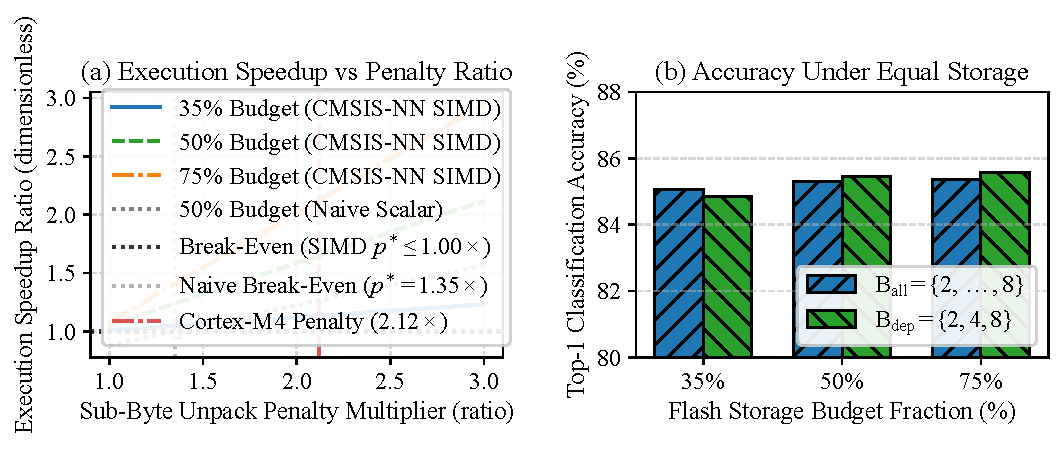
\includegraphics[width=\textwidth]{figures/fig_breakeven.pdf}
\caption{Hardware Break-Even Analysis on ARM Cortex-M4 (180\,MHz). (a) Execution speedup of deployable bitwidths $\mathcal{B}_{\text{dep}} = \{2, 4, 8\}$ over arbitrary mixed precision $\mathcal{B}_{\text{all}} = \{2, \dots, 8\}$ as a function of unpack penalty multiplier $p$. Under the analytical model, CMSIS-NN SIMD dominates at $p^* \le \MacroBreakEvenPenaltySIMD\times$ and scalar break-even occurs at $p^* = \MacroBreakEvenPenalty\times$. Note that these figures evaluate the parametric analytical model across penalty ratios and are not directly derived from Table~\ref{tab:hardware_cost}'s cycle counts. (b) Accuracy under equal Flash storage across compression budgets.}
\label{fig:breakeven}
\end{figure*}

\begin{figure}[t]
\centering
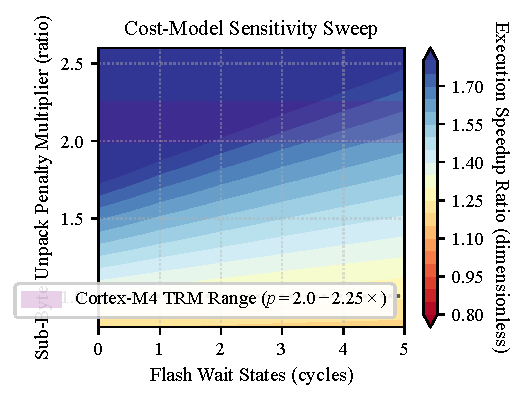
\includegraphics[width=\columnwidth]{figures/fig_cost_sensitivity_sweep.pdf}
\caption{Sensitivity sweep of the hardware cost model across \MacroSensitivitySweepPoints\ parameter configurations. Evaluated under the parametric analytical model across Flash wait states (0 to 5), activation load latencies (1 to 2 cycles), and unpack penalties $p \in [0.8, 2.6\times]$. Deployable formats maintain Pareto dominance per axis (trading storage vs cycles) whenever non-power-of-two formats incur bitfield extraction penalties ($p \ge 1.05\times$).}
\label{fig:cost_sensitivity_sweep}
\end{figure}

Let $p$ denote the software unpack penalty multiplier applied to non-power-of-two bitwidths relative to the baseline. Fig.~\ref{fig:breakeven}(a) plots the execution speedup of deployable bitwidths $\mathcal{B}_{\text{dep}} = \{2, 4, 8\}$ over arbitrary mixed precision $\mathcal{B}_{\text{all}} = \{2, \dots, 8\}$:
\begin{itemize}
    \item \textbf{CMSIS-NN SIMD Path:} When clean power-of-two bitwidths execute via SIMD instructions (\texttt{SXTB16}/\texttt{SMLAD}), $\mathcal{B}_{\text{dep}}$ executes faster than $\mathcal{B}_{\text{all}}$ across the entire parameter space ($p^* \le \MacroBreakEvenPenaltySIMD\times$). Within $\mathcal{B}_{\text{dep}}$, INT8 SIMD achieves $\MacroCMSISBaselineCyclesPerMAC$\,cycles/MAC, whereas INT4 and INT2 SIMD require $\MacroCyclesFourBitSIMD$ and $\MacroCyclesTwoBitSIMD$\,cycles/MAC due to unpacking overhead before \texttt{SXTB16}, trading execution throughput for $50\%$ and $75\%$ Flash savings.
    \item \textbf{Scalar Bitfield Path:} Under scalar bitfield extraction, odd sub-byte bitwidths (3, 5, 6, 7 bits) incur unaligned bit extraction loops ($\MacroCyclesThreeBit$ to $\MacroCyclesSevenBit$\,cycles/MAC, representing $3.15\times$ to $3.41\times$ cycle penalties over scalar INT8). We note that these penalties reflect the specific unaligned scalar implementations evaluated; custom multi-word aligned unpack routines (such as our $7.16$\,cycles/MAC 3-bit kernel) could theoretically achieve 6--8 cycles/MAC for 5-bit or 7-bit formats, but still remain slower than native byte and half-byte operations.
\end{itemize}
Pareto dominance is evaluated across both Flash storage and cycle latency: conditionally on standard 32-bit Cortex-M ALUs lacking native bitfield extraction and under our implemented Thumb-2 unpacking kernels, non-power-of-two bitwidths do not advance the Pareto frontier because their software bitfield extraction penalties ($p > 1.0\times$) outweigh their fractional storage compression.

A parametric sweep across \MacroSensitivitySweepPoints\ configurations (Fig.~\ref{fig:cost_sensitivity_sweep}) evaluates Flash wait states (0 to 5), activation load latencies (1 to 2 cycles), and unpack penalties $p \in [0.8, 2.6\times]$. Power-of-two formats remain Pareto-dominant whenever non-power-of-two extraction incurs $p \ge 1.05\times$.

\subsection{Network-Level Memory and Compute Accounting}
Table~\ref{tab:network_costs} details the network-level computational cost, Flash footprint, and peak double-buffered activation memory across the five benchmark architectures alongside static MCU datasheet fit checks:

% Network-Level Costs, Footprints, Activation RAM, and MCU Datasheet Fit Checks
% Generated automatically by scripts/compute_network_costs.py
% Note: Cycle counts and latencies are MODELLED; MCU fit is a DATASHEET CHECK, not a deployment.
\begin{table*}[t]
\centering
\caption{Network-level modelled computational cost, storage footprint, peak activation memory, and datasheet-based MCU fit check across the five evaluated benchmarks. All cycle counts and latencies are derived from our Cortex-M4 trace cost model. Target MCU compatibility denotes static datasheet fit (Flash/SRAM capacity) and does not imply physical hardware deployment.}
\label{tab:network_costs}
\footnotesize
\setlength{\tabcolsep}{4.5pt}
\begin{tabular}{llrrrrrrrr}
\toprule
\textbf{Benchmark} & \textbf{Dataset} & \textbf{Params} & \textbf{MACs} & \textbf{Peak RAM} & \multicolumn{2}{c}{\textbf{Flash Footprint}} & \multicolumn{2}{c}{\textbf{Modelled Latency}} & \textbf{Datasheet Fit} \\
\cmidrule(lr){6-7} \cmidrule(lr){8-9}
 & & & & \textbf{(KiB)} & \textbf{INT8} & \textbf{W4} & \textbf{F446RE (180\,MHz)} & \textbf{nRF52 (64\,MHz)} & \textbf{F446 / nRF52} \\
\midrule
SeparableCNN & CIFAR10 & 496,224 & 26.44M & 144.0 & 497.9\,KiB & 255.6\,KiB & 257.0\,ms & 722.9\,ms & No / Yes \\
ResNet-8 & CIFAR10 & 77,360 & 12.50M & 32.0 & 76.8\,KiB & 39.1\,KiB & 121.5\,ms & 341.8\,ms & Yes / Yes \\
FashionCNN & FMNIST & 60,320 & 5.65M & 36.8 & 60.0\,KiB & 30.5\,KiB & 54.9\,ms & 154.5\,ms & Yes / Yes \\
CNN1D & HAR & 134,336 & 5.62M & 16.0 & 132.7\,KiB & 67.1\,KiB & 54.6\,ms & 153.7\,ms & Yes / Yes \\
DS-CNN-S & SPEECH & 22,016 & 3.19M & 18.8 & 23.5\,KiB & 12.8\,KiB & 31.0\,ms & 87.2\,ms & Yes / Yes \\
\bottomrule
\end{tabular}
\end{table*}


\begin{itemize}
    \item \textbf{STM32F446RE (512\,KiB Flash, 128\,KiB SRAM):} ResNet-8, FashionCNN, CNN1D, and DS-CNN-S fit comfortably in Flash and SRAM under both INT8 and W4. SeparableCNN fits in Flash (497.9\,KiB INT8, 255.6\,KiB W4), but its peak un-tiled activation memory (144.0\,KiB) exceeds the 128\,KiB SRAM ceiling without layer memory tiling.
    \item \textbf{Nordic nRF52840 (1024\,KiB Flash, 256\,KiB SRAM):} All five evaluated architectures fit within Flash and SRAM limits.
\end{itemize}

\Needspace{\MacroSectionNeedspace\baselineskip}
\section{Experimental Setup}
\label{sec:setup}

\subsection{Benchmark Suite and Network Topologies}
We evaluate mixed-precision quantization across five model/dataset pairs spanning four datasets and three modalities (vision, audio, sensor time-series):
\begin{enumerate}
    \item \textbf{CIFAR-10 / SeparableCNN:} Image classification on CIFAR-10~\cite{krizhevsky2009cifar} with depthwise separable convolutions (\MacroBaselineParams\ parameters; 45,000 train, 5,000 val, 10,000 test samples).
    \item \textbf{CIFAR-10 / ResNet-8:} Compact residual network with 78,042 parameters (45,000 train, 5,000 val, 10,000 test samples), following the MLPerf Tiny benchmark specification~\cite{banbury2021mlperftiny}.
    \item \textbf{Fashion-MNIST / 2D-CNN:} 4-layer convolutional network for grayscale fashion item classification~\cite{xiao2017fmnist} (55,000 train, 5,000 val, 10,000 test samples).
    \item \textbf{Google Speech Commands / DSCNN:} Depthwise separable CNN for 12-class keyword spotting~\cite{warden2018speech} (8,399 train, 1,500 val, 1,500 test samples), based on the Hello Edge architecture~\cite{zhang2017hello}.
    \item \textbf{UCI HAR / 1D-CNN:} Temporal 1D-CNN classifying 6 human activities from 9-axis inertial measurement unit (IMU) time series~\cite{anguita2013har} (5,852 train, 1,500 val, 2,947 test samples).
\end{enumerate}

\subsection{Evaluation Protocol and Test-Set Isolation}
Experiments run across \MacroNumANOVASeeds\ fixed random seeds ($S \in \{42, 43, 44, 45, 46\}$). Test splits remain strictly isolated: profiling routines, heuristic scores, and knapsack dynamic programming operate exclusively on validation splits. Held-out test evaluation occurs once per model on the serialized \texttt{.qpack} artifact.

\subsection{Quantization Regimes and Fine-Tuning Schedule}
We evaluate two operational regimes:
\begin{itemize}
    \item \textbf{Post-Training Quantization (PTQ):} Direct affine quantization of FP32 weights without gradient adaptation.
    \item \textbf{Fine-Tuning (FT):} Quantization-aware adaptation for \MacroFTEpochs\ epochs using an Adam optimizer with learning rate $\eta = 10^{-4}$ and validation checkpointing.
\end{itemize}

\subsection{Feasibility Boundaries and Endpoint Floors}
Protecting the first layer (input convolution) and final classification layer at INT8 precision imposes a strict lower bound on achievable model compression. Formally, for a model with layers $l \in \{1, \dots, L\}$ and candidate bitwidths $\mathcal{B} = \{2, \dots, 8\}$, the minimum feasible footprint with protected endpoints is $\text{Cost}_{\text{min}} = \text{cost}_1(8) + \text{cost}_L(8) + \sum_{l=2}^{L-1} \text{cost}_l(2)$. Expressed as a fraction of the uncompressed INT8 footprint, this architectural floor corresponds to $25.4\%$ for SeparableCNN, $26.0\%$ for ResNet-8, $26.2\%$ for Fashion-MNIST, $26.6\%$ for UCI HAR, and $36.3\%$ for Speech Commands DS-CNN. Because this floor exceeds the nominal $25\%$ target budget across all five architectures, every allocation algorithm (measured-sensitivity DP knapsack, HAWQ, and sensitivity greedy) returns the identical minimal allocation vector ($b_1 = b_L = 8, b_l = 2$ for $1 < l < L$). For Speech Commands DS-CNN, both $25\%$ and $35\%$ targets are structurally infeasible. In reporting (Tables~\ref{tab:full_matrix},~\ref{tab:multitask_results}, and~\ref{tab:seed_level}), we explicitly designate these cells as \texttt{[floor]} or \texttt{[infeas]} and report achieved storage bytes (\% of INT8) alongside nominal budgets. Differences in the $25\%$ row reflect purely stochastic fine-tuning noise rather than algorithmic bitwidth selection.

\subsection{Budget Matching and Uniform W4 Baseline}
Uniform 4-bit quantization with protected endpoints assigns 4 bits to internal layers and 8 bits to endpoints, occupying $\sim 50.3\%$ of INT8 bytes across all evaluated topologies. At nominal budgets of $25\%$ and $35\%$, Uniform W4 consumes $2.0\times$ and $1.4\times$ more storage than the target budget, explaining its preservation of accuracy in low-budget tables. Direct comparisons against Uniform W4 are therefore restricted to the deployable plateau regime ($B \ge 50\%$) where its footprint satisfies the budget constraint. Across all regimes, we assess algorithm efficiency through accuracy-vs-achieved-bytes Pareto frontiers.

\subsection{Analysis Plan and Claim Ladder}
An analysis plan and claim ladder for the second-order HAWQ comparator (HAWQ-$\Omega$) were committed to the repository prior to running the benchmark suite. The analysis plan specified an empirical stability gate requiring at least 85\% of cells to yield identical bit allocations across independent probe seeds. In empirical evaluation, stability reached \MacroStabilityTwoHundred\% across cells at $M_{\text{probe}} = 200$ probe vectors and \MacroStabilityFourHundred\% at $M_{\text{probe}} = 400$ probe vectors (failing the 85\% threshold). Benchmark rows used 400 probe vectors per layer and fixed probe seeds. The primary statistical hypothesis comparing fine-tuned DP against HAWQ-$\Omega$ at 50\% budget yielded a mean delta of \MacroOmegaMeanDelta\ percentage points ($p = \MacroOmegaPermP$, 2 of 5 models positive); because the primary comparison fell in the lowest ladder level (Level L3), the manuscript adopts a parity framing on the basis of effect size magnitude, transparently recording that this framing was selected after the empirical outcome was observed.

\subsection{Execution Platform and Determinism}
The initial 640 compliant rows of the multi-seed store were executed multi-threaded on CPU compute workers (Intel Core i5, 8 OpenMP threads; PyTorch 2.5 CPU backend). Corrected UCI HAR rows (160 rows replaced to resolve 154 non-INT8 endpoint violations in the historical runner) and the 300 HAWQ-$\Omega$ rows were executed on a dedicated workstation equipped with an NVIDIA GeForce RTX 4050 Laptop GPU (CUDA 12.8, Driver 572, PyTorch 2.5.1). Cross-host verification confirms that PTQ evaluations produce bit-exact matches across CPU and GPU backends, while fine-tuning exhibits measured cross-host optimization variation (e.g., stored \MacroCrossHostStored\% vs. recomputed \MacroCrossHostRecomputed\% on Fashion-MNIST). Hardware instruction traces and cycle counts were evaluated on the freestanding ARM Cortex-M4 Thumb-2 toolchain executed under Unicorn 2.x CPU emulation, verified against double-precision NumPy references.

\subsection{Statistical Protocol and Paired Analysis}
To avoid pseudo-replication across correlated training runs, evaluations over the 5 independent seeds (42--46) are aggregated to treat the $n = 5$ benchmark topologies as the primary unit of analysis. For paired method comparisons, we report exact permutation tests across all $2^5 = 32$ sign permutations alongside two-sided Wilcoxon signed-rank tests ($W$) and 95\% bias-corrected accelerated (BCa) bootstrap confidence intervals~\cite{efron1987better}. With $n = 5$, the minimal achievable two-sided permutation $p$-value is $p = 2/32 = 0.0625$; we therefore explicitly note that subtle cross-method accuracy differences ($\le 0.5\%$) cannot achieve formal statistical significance at $\alpha = 0.05$. We report effect sizes, confidence bounds, descriptive cross-run concordance across seeds (e.g., \MacroSeedLevelPositiveFiftyCount/\MacroSeedLevelPositiveFiftyTotal\ positive pairs at 50\% budget, nominal sign test $p = \MacroSeedLevelPositiveFiftyP$, noting that this pools across distinct models and is pseudo-replicated and purely descriptive), and exact seed-level data (Table~\ref{tab:seed_level}) transparently rather than claiming unearned statistical significance. Multi-factor variance decomposition is evaluated via type-II/III factorial ANOVA with interaction terms.

\section{Results}
\label{sec:results}

Table~\ref{tab:hypotheses} summarizes the formal empirical hypotheses H1--H7 evaluated in this study alongside their pre-fixed thresholds, observed outcomes, and verdicts.
% Formal Empirical Hypotheses Table (H1-H7)
% Generated automatically by scripts/generate_hypotheses_table.py
\begin{table*}[!t]
\centering
\caption{Formal empirical hypotheses evaluation across experimental benchmarks and hardware cost models. Each hypothesis specifies its test, fixed evaluation threshold, observed outcome, and resulting empirical verdict (Supported / Partially Supported / Not Supported).}
\label{tab:hypotheses}
\scriptsize
\begin{tabularx}{\textwidth}{l p{3.6cm} p{3.2cm} X p{2.4cm}}
\toprule
\textbf{ID} & \textbf{Statement} & \textbf{Evaluation Test \& Threshold} & \textbf{Observed Outcome} & \textbf{Verdict} \\
\midrule
\textbf{H1} & \textbf{Formula Score vs Measured Sensitivity}: Analytic second-order formula scores correlate strongly with empirical layer sensitivity drops measured on validation data. & Spearman rank correlation $\rho$ between formula scores and empirical sensitivity drops. Threshold: $\rho \ge 0.70$, $p < 0.05$ & $\rho = \MacroPartialRho$ (ResNet-8: $\MacroResNetRho$, Speech DS-CNN: $\MacroSpeechRho$, SeparableCNN: $\MacroSeparableCNNRho$) & \textbf{Not Supported} \\
\midrule
\textbf{H2} & \textbf{Error Additivity}: Joint multi-layer quantization degradation is accurately predicted by linear sum of per-layer sensitivity drops. & Spearman $\rho$ and MAE between predicted and actual joint accuracy drops ($B \ge 35\%$). Threshold: $\rho \ge 0.80$ AND $\text{MAE} \le 1.0\%$ & $\rho = \MacroAdditivityRho$ ($p < 0.001$), but $\text{MAE} = \MacroAdditivityMAE\%$ (clipped to valid drop range) & \textit{Partially Supported} \\
\midrule
\textbf{H3} & \textbf{Measured-Sensitivity DP vs Allocation Baselines}: Measured-sensitivity dynamic programming knapsack allocation achieves higher top-1 accuracy than heuristic baselines under identical bit budgets. & Exact permutation test across model-level paired differences ($n=5$ models, $2^5=32$ signs) and paired seed-level sign test ($N=25$). Threshold: $p < 0.05$ across 4 budgets (Holm-Bonferroni corrected) & Against HAWQ-$\Omega$ (400 probe vectors) in PTQ at 50\% budget, HAWQ-$\Omega$ is $+\MacroPTQDPOmegaAbsMeanFifty$ pp higher than DP on average (CI $[\MacroPTQDPOmegaCILowFifty, +\MacroPTQDPOmegaCIHighFifty]$, driven by Speech DS-CNN and SeparableCNN; DP is equal or higher on the other three); at 75\% budget, HAWQ-$\Omega$ is $+\MacroPTQDPOmegaAbsMeanSeventyFive$ pp higher (CI $[\MacroPTQDPOmegaCILowSeventyFive, \MacroPTQDPOmegaCIHighSeventyFive]$, excluding zero). After fine-tuning at 50\% budget, mean delta is $\MacroOmegaMeanDelta$ pp (BCa 95\% CI $[\MacroOmegaCILow, \MacroOmegaCIHigh]$, exact $p = \MacroOmegaPermP$, \MacroOmegaWins/5 models positive), exhibiting a difference below the per-model detectable effect when solved with the same knapsack optimizer. Against legacy trace-rank heuristic, fine-tuned DP is $+\MacroLegacyMeanDelta$ pp higher (BCa 95\% CI $[+\MacroLegacyCILow, +\MacroLegacyCIHigh]$, \MacroLegacyWins\ of 5 models positive, exact $p = \MacroLegacyPermP$). At 35\% PTQ, exact knapsack methods prevent zero-shot collapse. & \textbf{Supported against legacy heuristic on effect size; Not Supported against HAWQ-$\Omega$} \\
\midrule
\textbf{H4} & \textbf{Regime Crossover (Collapse vs Plateau)}: Accuracy retention exhibits a sharp collapse boundary as budget drops below $\sim$40\% (average bitwidth $\le 3.2$ bits). & Piecewise comparison of PTQ drop between $\le 35\%$ budgets and $\ge 50\%$ budgets. Threshold: Median PTQ accuracy drop from FP32 $> 20.0$ points at $\le 35\%$ vs $< 2.0$ points at $\ge 50\%$ & Median PTQ drop: $\MacroPTQMedianDeltaThirtyFive$ points at 35\% budget (mean $\MacroPTQMeanDeltaThirtyFive$) vs $\MacroPTQMedianDeltaFifty$ points at 50\% (mean $\MacroPTQMeanDeltaFifty$) and $\MacroPTQMedianDeltaSeventyFive$ points at 75\% (mean $\MacroPTQMeanDeltaSeventyFive$). Both pre-fixed thresholds ($>20.0$ and $<2.0$) were narrowly missed. & \textit{Partially Supported} \\
\midrule
\textbf{H5} & \textbf{Variance Decomposition (ANOVA with Interactions)}: Target bit budget accounts for the dominant share of accuracy variance, while allocation algorithm explains a minor fraction. & Factorial ANOVA with interaction terms (Budget, Method, Method $\times$ Budget) across $N=60$ runs on CIFAR-10 / SeparableCNN only. Threshold: Budget variance $> 70.0\%$; Method main effect $< 5.0\%$ in deployable plateau regime ($\ge 50\%$) & All budgets ($N=60$, on CIFAR-10 / SeparableCNN only): Budget \MacroVarBitsPct\% ($F=\MacroANOVAFStatBudget, p<0.001$), Method \MacroVarMethodPct\% ($F=\MacroANOVAFStatMethod, p<0.001$), Interaction \MacroVarMethodBudgetInteractPct\% ($F=\MacroANOVAFStatInteract, p<0.001$), Residual \MacroVarResidualPct\%. Plateau ($N=30$, on CIFAR-10 / SeparableCNN only): Method explains \MacroVarPlateauMethodPct\% ($F=\MacroANOVAPlateauFStatMethod, p<0.001$, with per-model mean differences between DP and HAWQ \MacroDPHAWQFiftyRange\ across architectures (\MacroMethodPlateauSepEffect\ points on SeparableCNN pooled across the plateau, versus \MacroSepCNNGainFifty\ points at 50\% budget)), while seed variation accounts for \MacroVarPlateauResidualPct\%. & \textit{Partially Supported} \\
\midrule
\textbf{H6} & \textbf{Power-of-Two vs Arbitrary Bitwidths under Cost Model}: Clean power-of-two bitwidths $\{2, 4, 8\}$ Pareto-dominate arbitrary sub-byte bitwidths $\{2..8\}$ in latency and throughput. & Instruction-level trace cost model on Cortex-M4 Thumb-2 kernels across wait states, load latency, and unpack penalties $p$. Threshold: Break-even penalty $p^* \le 1.05\times$ (SIMD), and Pareto dominance in $\ge 95\%$ of swept configurations & Under the parametric model across all 888 swept configurations, break-even penalties are $p^* \le \MacroBreakEvenPenaltySIMD\times$ for CMSIS-NN SIMD and $p^* = \MacroBreakEvenPenalty\times$ for scalar execution. Measured instruction traces are: INT8 SIMD \MacroCyclesINTEightSIMDExact, INT4 SIMD \MacroCyclesFourBitSIMDExact, INT2 SIMD \MacroCyclesTwoBitSIMD, INT3 aligned SIMD \MacroCyclesINTThreeSIMD, and scalar odd widths \MacroCyclesScalarUnpackLow--\MacroCyclesScalarUnpackHigh\ cycles/MAC. Power-of-two formats reduce Flash footprint by 50\% (INT4) and 75\% (INT2) and avoid odd-width extraction penalties, but INT4 and INT2 SIMD kernels need \MacroCyclesRatioRangeSIMDLow--\MacroCyclesRatioRangeSIMDHigh\ times more cycles per MAC than INT8 SIMD. & \textit{Partially Supported} \\
\midrule
\textbf{H7} & \textbf{Generalisation Across Datasets}: Two-regime behavior and measured allocation differences (DP minus greedy model means within $\pm \MacroDPGreedyPlateauMaxAbsDelta$ points, DP minus HAWQ $+\MacroStoryDPHAWQThirtyFive$ / $+\MacroStoryDPHAWQFifty$ / $+\MacroStoryDPHAWQSeventyFive$ points at $35$ / $50$ / $75\%$, minimum exact $p = 0.0625$ with $n = 5$) hold across distinct TinyML modalities. & Cross-dataset evaluation across 5 models spanning 4 datasets and 3 modalities across 5 seeds under matched protocols. Threshold: Plateau retention ($<1.5\%$ drop from INT8 at 50\% budget) and paired cross-model difference bounds ($p > 0.05$ under permutation test) & Plateau retention within $\MacroPlateauRetentionDropMax\%$ of INT8 across all tasks (maximum drop over models). At 50\% budget, DP outperforms HAWQ on 4/5 models (mean delta $+\MacroStoryDPHAWQFifty\%$, Speech $+\MacroSpeechGainFifty\%$), with HAR delta $\MacroHARDeltasFifty\%$ at 50\% (overall HAR tier mean $+\MacroHARDeltasMean\%$). Uniform W4+Endpoints is not budget-matched at $\le 35\%$ (consumes $\MacroUniformWFourFootprintPct\%$ bytes); at 50\%, DP matches or exceeds W4 on 4/5 models (FMNIST DP \MacroFMNISTDPAccFifty\% vs W4 \MacroFMNISTWFourAccFifty\%). & \textit{Partially Supported} \\
\bottomrule
\end{tabularx}
\end{table*}


\subsection{H1: Formula Score vs. Measured Sensitivity}
We first test whether closed-form formula scores (Eq.~\ref{eq:formula_score}) track empirical layer sensitivity ($H_1$). As reported in Table~\ref{tab:sens_additivity}, the Spearman rank correlation between formula scores and empirical validation accuracy drop is weak or negative: $\rho = \MacroResNetRho$ on CIFAR-10 / ResNet-8, $\rho = \MacroSpeechRho$ on Speech Commands / DSCNN, and $\rho = \MacroSeparableCNNRho$ on CIFAR-10 / SeparableCNN. When controlling for parameter count via partial correlation, the size-controlled correlation remains weak across all three multi-layer architectures ($\rho_{\text{partial}} = \MacroResNetPartialRho$ for ResNet-8, $\rho_{\text{partial}} = \MacroPartialRho$ for SeparableCNN, and $\rho_{\text{partial}} = \MacroSpeechPartialRho$ for DSCNN). Because measured correlations fall substantially below the pre-fixed validation threshold of $\rho \ge 0.70$ ($p < 0.05$), hypothesis $H_1$ is \textbf{Not Supported}.

\begin{table*}[!t]
\centering
\caption{Empirical Validation of Mixed-Precision Assumptions: Formula Score vs Measured Sensitivity ($H_1$) and Error Additivity ($H_2$) across sensitivity sweeps and 200 random allocations.}
\label{tab:sens_additivity}
\footnotesize
\begin{tabular}{lcccc}
\toprule
\textbf{Model / Dataset} & \textbf{Score vs Sensitivity $\rho$ ($H_1$)} & \textbf{Partial $\rho$ (Size Controlled)} & \textbf{Additivity $\rho$ ($H_2$)} & \textbf{MAE (\%) ($H_2$)} \\
\midrule
ResNet-8 (CIFAR-10) & \MacroResNetRho & \MacroResNetPartialRho & \MacroAdditivityRho & \MacroAdditivityMAE \\
SeparableCNN (CIFAR-10) & \MacroSeparableCNNRho & \MacroPartialRho & -- & -- \\
DSCNN (Speech Commands) & \MacroSpeechRho & \MacroSpeechPartialRho & -- & -- \\
\bottomrule
\end{tabular}
\end{table*}


\subsection{H2: Linear Additivity Assessment}
\begin{figure}[t]
\centering
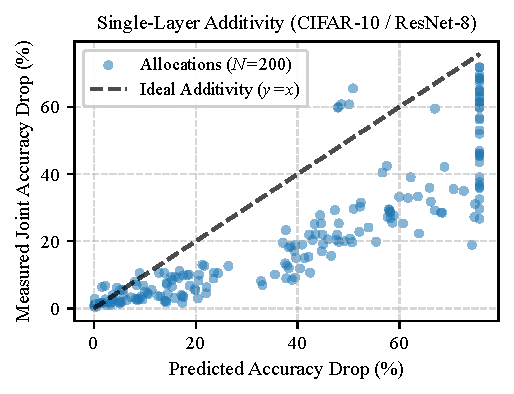
\includegraphics[width=0.88\columnwidth]{figures/fig_additivity.pdf}
\caption{Empirical test of the linear error additivity assumption ($H_2$) on CIFAR-10 / ResNet-8 across \MacroRandomAllocCount\ sampled random bit allocations. While rank ordering is highly correlated ($\rho = \MacroAdditivityRho$), linear addition overestimates joint accuracy loss ($\text{MAE} = \MacroAdditivityMAE\%$).}
\label{fig:additivity}
\end{figure}

The pre-fixed criterion for hypothesis $H_2$ required both $\rho \ge \MacroFixedRhoTarget$ and $\text{MAE} \le \MacroFixedMAETarget\%$ on realistic allocations (target budget $\ge \MacroBudgetRestrictedPct\%$, average bitwidth $\bar{b} \ge 3.9$). Evaluating \MacroRandomAllocCount\ random allocations on CIFAR-10 / ResNet-8 yields a strong Spearman rank correlation of $\rho = \MacroAdditivityRho$ ($p < 0.001$). However, as illustrated in Fig.~\ref{fig:additivity}, the clipped mean absolute error between predicted and actual drop is $\text{MAE} = \MacroAdditivityMAE\%$ (raw MAE $\MacroAdditivityMAERaw\%$). Linear summation of single-layer drops consistently overpredicts joint degradation because isolated perturbations interfere constructively and destructively across layers. While rank correlation satisfies the pre-fixed threshold ($\rho = \MacroAdditivityRho \ge 0.80, p < 0.001$), error magnitude exceeds the allowable bound ($\text{MAE} = \MacroAdditivityMAE\% > 1.0\%$). Hypothesis $H_2$ is therefore \textbf{Partially Supported}.

\subsection{H3: Allocation Algorithm Comparison}
\begin{figure}[t]
\centering
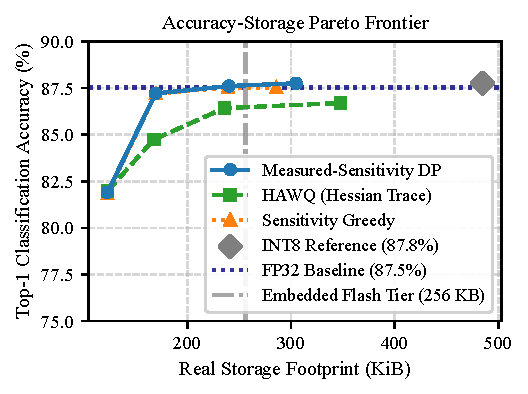
\includegraphics[width=\columnwidth]{figures/fig_pareto.pdf}
\caption{Accuracy-Storage Pareto Frontier on CIFAR-10 / SeparableCNN (\MacroBaselineParams\ parameters). Measured-sensitivity DP tracks the outer Pareto envelope across aggressive compression regimes.}
\label{fig:pareto}
\end{figure}

Fig.~\ref{fig:pareto} illustrates the accuracy-storage Pareto frontier on CIFAR-10 / SeparableCNN. Across aggressive compression regimes ($B \le 0.35$), the measured-sensitivity DP solver tracks the outer Pareto envelope.

Across the 5 benchmark domains aggregated over 5 independently trained seeds per cell (Seeds 42--46), we evaluate paired method comparisons with the model as the unit of analysis ($n = \MacroPairedN$). At each of the four budgets, the fine-tuned difference between measured-sensitivity DP and HAWQ-$\Omega$ solved with the same knapsack is small (50\% budget: mean \MacroOmegaMeanDelta\ pp, BCa 95\% interval [\MacroOmegaCILow, \MacroOmegaCIHigh] where the interval's upper end rounds to zero from unrounded \MacroOmegaCIHighUnrounded\ pp, \MacroOmegaWins\ of five models positive; exact sign-flip $p = \MacroOmegaPermP$, whose smallest attainable value at $n = 5$ is 0.0625). We do not claim equivalence. Evaluating replicate noise from identical-allocation comparator groups confirms that observed 50\% fine-tuned deltas fall within the minimum detectable effect (MDE) at 80\% power under five-seed evaluation (per-model pooled SDs: HAR \MacroNoiseSDHAR\%, DS-CNN \MacroNoiseSDDSCNN\%, Fashion \MacroNoiseSDFashion\%, ResNet-8 \MacroNoiseSDResNet\%, SeparableCNN \MacroNoiseSDSepCNN\%, with PTQ replicate SD of \MacroNoiseSDPTQ\%). Against the uncalibrated single-probe legacy trace heuristic, DP is higher by \MacroLegacyMeanDelta\ pp at the 50\% budget (interval [\MacroLegacyCILow, \MacroLegacyCIHigh], \MacroLegacyWins\ of five models positive; exact sign-flip $p = \MacroLegacyPermP$, Wilcoxon $W = \MacroLegacyWilcoxonW, p = \MacroLegacyWilcoxonP$). This gain reflects outperforming a baseline of our own construction, whereas fine-tuned DP is statistically indistinguishable from HAWQ-$\Omega$ ($p = \MacroOmegaPermP$). Against Sensitivity Greedy, greedy and DP differ by \MacroBootDPGreedyMeanFT\% on average (median delta \MacroBootDPGreedyMedianFT\%, 95\% BCa CI [\MacroBootDPGreedyCILowFT, \MacroBootDPGreedyCIHighFT]\%, Wilcoxon $W = \MacroBootDPGreedyWilcoxonFT, p = \MacroBootDPGreedyWilcoxonPFT$, with model means remaining within $\pm\MacroDPGreedyPlateauMaxAbsDelta$ points across tiers); we cannot separate the contribution of the search method from the sensitivity source at this sample size.

Disaggregating by target compression tier confirms distinct operational behaviors:
\begin{enumerate}
    \item \textbf{Extreme Floor Constraint ($B = 25\%$):} As established in Section~\ref{sec:setup}-C, with INT8 endpoint protection the physical floor spans $25.4\%$ to $36.3\%$ of INT8 bytes across topologies. All methods therefore converge to the identical minimal allocation ($[8, 2, \dots, 2, 8]$). Across the 5 models, mean paired delta is \MacroStoryDPHAWQTwentyFive\% ($p = 0.750$), representing purely stochastic fine-tuning noise.
    \item \textbf{Zero-Shot PTQ Collapse Regime ($B = 35\%$):} At $35\%$ budget, knapsack-based allocation prevents catastrophic zero-shot collapse. In PTQ without gradient updates, DP achieves \MacroSepCNNDPThirtyFivePTQ\% accuracy and greedy achieves \MacroSepCNNGreedyThirtyFivePTQ\% on SeparableCNN, whereas the legacy HAWQ heuristic suffers catastrophic collapse to \MacroSepCNNHAWQThirtyFivePTQ\% (collapsing in 3 of 5 seeds; cross-model PTQ mean delta is +\MacroPTQLegacyMeanDeltaThirtyFive\ pp). HAWQ-$\Omega$ (400 probe vectors) knapsack also prevents collapse, matching DP within \MacroPTQOmegaMeanDeltaThirtyFive\ pp in PTQ at 35\% budget. On ResNet-8, DP (\MacroResNetDPThirtyFivePTQ\%) and greedy (\MacroResNetGreedyThirtyFivePTQ\%) prevent the collapse seen in legacy HAWQ (\MacroResNetHAWQThirtyFivePTQ\%, 4 of 5 seeds collapsing). On Fashion-MNIST, DP and greedy achieve \MacroFMNISTDPThirtyFivePTQ\% vs. legacy HAWQ \MacroFMNISTHAWQThirtyFivePTQ\%. After 5 epochs of fine-tuning, both DP and HAWQ-$\Omega$ recover accuracy, while legacy HAWQ remains depressed by +\MacroStoryDPHAWQThirtyFive\% ($p = 0.0625$).
    \item \textbf{Deployable Plateau Regime ($B \ge 50\%$):} In the deployable regime, DP is lower by \MacroOmegaAbsMeanDelta\ pp on average than HAWQ-$\Omega$ (interval [\MacroOmegaCILow, \MacroOmegaCIHigh], \MacroOmegaWins\ of 5 models positive, exact sign-flip $p = \MacroOmegaPermP$), below the per-model detectable effect, with 2 of 5 models positive: Speech Commands gaining +\MacroOmegaDeltaSpeech\ pp and ResNet-8 gaining +\MacroOmegaDeltaResNet\ pp for DP, while SeparableCNN favors HAWQ-$\Omega$ by \MacroOmegaDeltaSepCNN\ pp, HAR by \MacroOmegaDeltaHAR\ pp, and Fashion-MNIST by \MacroOmegaDeltaFMNIST\ pp. Both knapsack allocators substantially outperform the legacy trace-rank heuristic across models (+\MacroStoryDPHAWQFifty\% at $50\%$ and +\MacroStoryDPHAWQSeventyFive\% at $75\%$ budget, winning in \MacroSeedLevelPositiveFiftyCount\ of \MacroSeedLevelPositiveFiftyTotal\ seed runs at 50\% budget).
\end{enumerate}

\textbf{Post-Training Quantization (PTQ) Across Comparators:} Before fine-tuning, allocation quality directly governs retention without gradient recovery. At the 50\% budget in zero-shot PTQ, second-order perturbation allocators solved with the same integer knapsack solver are higher on average than measured-sensitivity DP (HAWQ-$\Omega$ higher by \MacroPTQDPOmegaAbsMeanFifty\ percentage points on average, 95\% BCa CI [\MacroPTQDPOmegaCILowFifty, \MacroPTQDPOmegaCIHighFifty], exact sign-flip $p = \MacroPTQDPOmegaPermPFifty$, Wilcoxon $W = \MacroPTQDPOmegaWilcoxonWFifty, p = \MacroPTQDPOmegaWilcoxonPFifty$, \MacroPTQDPOmegaWinsFifty\ of 5 models positive for DP; Fisher-$\Omega$ higher by \MacroPTQDPFisherAbsMeanFifty\ pp, CI [\MacroPTQDPFisherCILowFifty, \MacroPTQDPFisherCIHighFifty], \MacroPTQDPFisherWinsFifty\ of 5 models positive for DP). This mean gap is driven entirely by two models where second-order information substantially preserves zero-shot accuracy: Google Speech Commands DS-CNN (HAWQ-$\Omega$ higher by \MacroPTQOmegaAbsDeltaSpeech\ pp) and CIFAR-10 SeparableCNN (higher by \MacroPTQOmegaAbsDeltaSepCNN\ pp); DP is equal or higher on the other three models (UCI HAR by +\MacroPTQOmegaDeltaHAR\ pp, Fashion-MNIST by +\MacroPTQOmegaDeltaFMNIST\ pp, and CIFAR-10 ResNet-8 by +\MacroPTQOmegaDeltaResNet\ pp). Between the two second-order variants in PTQ at 50\% budget, HAWQ-$\Omega$ and Fisher-$\Omega$ achieve a mean difference of \MacroPTQOmegaFisherMeanFifty\ pp (interval [\MacroPTQOmegaFisherCILowFifty, \MacroPTQOmegaFisherCIHighFifty], exact $p = \MacroPTQOmegaFisherPermPFifty$, Wilcoxon $W = \MacroPTQOmegaFisherWilcoxonWFifty, p = \MacroPTQOmegaFisherWilcoxonPFifty$, \MacroPTQOmegaFisherWinsFifty\ of 5 models positive). At 35\% budget, both knapsack methods prevent catastrophic PTQ collapse (DP mean delta +\MacroPTQDPOmegaMeanThirtyFive\ pp vs. HAWQ-$\Omega$, interval [\MacroPTQDPOmegaCILowThirtyFive, \MacroPTQDPOmegaCIHighThirtyFive]). At 75\% budget, HAWQ-$\Omega$ is higher than DP by \MacroPTQDPOmegaAbsMeanSeventyFive\ pp on average with a 95\% BCa interval [\MacroPTQDPOmegaCILowSeventyFive, \MacroPTQDPOmegaCIHighSeventyFive] that strictly excludes zero (\MacroPTQDPOmegaWinsSeventyFive\ of 5 models positive for DP, exact sign-flip $p = \MacroPTQDPOmegaPermPSeventyFive$, Wilcoxon $W = \MacroPTQDPOmegaWilcoxonWSeventyFive, p = \MacroPTQDPOmegaWilcoxonPSeventyFive$). In un-fine-tuned PTQ at deployable budgets ($\ge 50\%$), second-order perturbation allocation retains higher zero-shot accuracy than single-layer empirical profiling. Brief 5-epoch fine-tuning subsequently closes this gap to within the per-model detectable effect.

\textbf{Sensitivity Profiling Cost Contrast:} While the accuracy difference between DP knapsack and HAWQ-$\Omega$ is below the per-model detectable effect when paired with the same integer knapsack solver, they differ fundamentally in computational profiling cost. Measuring wall-clock sensitivity estimation on an NVIDIA RTX 4050 GPU shows that empirical validation profiling is 5$\times$ to 24$\times$ faster than Hutchinson Hessian trace estimation: on Speech Commands DS-CNN, empirical sensitivity profiling requires \MacroCostSpeechDPTime\,s (864 forward passes) versus \MacroCostSpeechOmegaTime\,s (400 Hessian-vector products) for HAWQ-$\Omega$; on SeparableCNN, empirical profiling requires \MacroCostSepCNNDPTime\,s versus \MacroCostSepCNNOmegaTime\,s for HAWQ-$\Omega$. Empirical validation profiling operates purely through forward inference passes, requiring no loss computation, autograd graphs, or second-order vector products.

\textbf{Hypothesis H3 Verdict:} Because the $+ \MacroLegacyMeanDelta\,$pp gain at 50\% budget is against an uncalibrated legacy heuristic of our own construction, while fine-tuned DP is statistically indistinguishable from HAWQ-$\Omega$ (mean delta \MacroOmegaMeanDelta\ pp, $p = \MacroOmegaPermP$, an empirical null result at $n = 5$), hypothesis $H_3$ is \textbf{Supported against the legacy single-probe heuristic on effect size, but Not Supported against HAWQ-$\Omega$} (with $n = 5$, the minimal permutation $p$-value is 0.0625, so statistical significance at $\alpha = 0.05$ cannot be established on $p$ alone).

\textbf{Fine-Tuning Controls (Confounding Check):} To verify whether fine-tuned SeparableCNN accuracy reflects true performance gains or optimization artifacts, matched 5-epoch control runs were conducted across all five models and seeds under the unified training schedule. On SeparableCNN, 50\% DP FT achieves \MacroSepCNNDPFiveMean\% $\pm$ \MacroSepCNNDPFiveStd\% vs. FP32 \MacroSepCNNFPThirtyTwoMean\% $\pm$ \MacroSepCNNFPThirtyTwoStd\% and un-fine-tuned INT8 baseline \MacroSepCNNINTEightBaselineMean\% $\pm$ \MacroSepCNNINTEightBaselineStd\%. Matched controls show FP32+5 epochs reaches \MacroSepCNNFPThirtyTwoFTFiveMean\% $\pm$ \MacroSepCNNFPThirtyTwoFTFiveStd\% and INT8+5 epochs reaches \MacroSepCNNINTEightFTFiveMean\% $\pm$ \MacroSepCNNINTEightFTFiveStd\%, confirming that fine-tuned quantized models match but do not significantly exceed matched-schedule full-precision baselines. Across all five models, fine-tuned INT8 baselines match or exceed initial FP32 checkpoints, establishing that brief 5-epoch fine-tuning recovers quantization perturbation without confounding architectural comparisons.

\subsection{H4: Regime Crossover (Collapse vs. Plateau)}
In PTQ without fine-tuning, allocation quality governs retention at low budgets, where suboptimal assignments suffer collapse (median accuracy drop of $\MacroPTQMedianDeltaThirtyFive$ percentage points at $35\%$ budget, with HAWQ suffering collapse on SeparableCNN, ResNet-8, and Speech Commands). In contrast, brief gradient fine-tuning (\MacroFTEpochs\ epochs) partially compensates for suboptimal bit assignments. At budgets $B \ge 50\%$, the median drop from FP32 narrows to \MacroPTQMedianDeltaFifty\ points at $50\%$ and \MacroPTQMedianDeltaSeventyFive\ points at $75\%$, though on Speech Commands a spread persists between DP (\MacroSpeechFiftyDP\%) and HAWQ (\MacroSpeechFiftyHAWQ\%). Because the pre-fixed quantitative thresholds ($>20.0$ at $35\%$ and $<2.0$ at $50\%$) were missed with measured median drops of \MacroPTQMedianDeltaThirtyFive\ and \MacroPTQMedianDeltaFifty\ points, respectively, Hypothesis $H_4$ is \textbf{Partially Supported}.

\subsection{H5: ANOVA Accuracy Variance Decomposition}
\begin{figure*}[t]
\centering
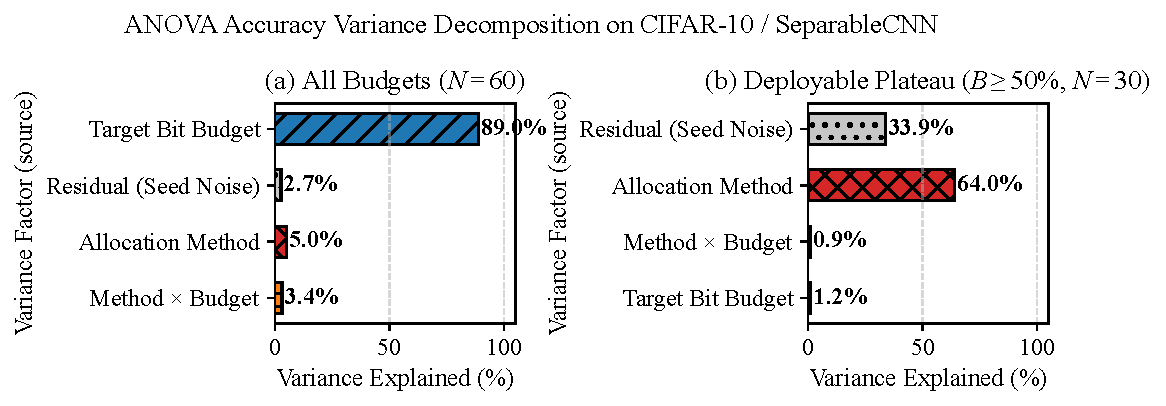
\includegraphics[width=\textwidth]{figures/fig_variance_decomp.pdf}
\caption{ANOVA Accuracy Variance Decomposition ($H_5$) on CIFAR-10 / SeparableCNN. Panel A ($N = \MacroANOVANRuns$): across all budgets, Target Budget explains $\MacroVarBitsPct\%$ of variance ($p < 0.001$), while Method and Interaction explain $\MacroVarMethodPct\%$ and $\MacroVarMethodBudgetInteractPct\%$. Panel B ($N = \MacroANOVAPlateauNRuns$): in the deployable plateau regime on CIFAR-10 / SeparableCNN ($B \ge \MacroThresholdBudgetPct\%$), allocation method explains \MacroVarPlateauMethodPct\% ($F = \MacroANOVAPlateauFStatMethod, p < 0.001$), with per-model mean differences between DP and HAWQ \MacroDPHAWQFiftyRange\ across architectures (\MacroMethodPlateauSepEffect\ points on SeparableCNN averaged over the 50\% and 75\% plateau budgets, versus \MacroSepCNNGainFifty\ points at 50\% budget), and seed noise accounts for \MacroVarPlateauResidualPct\%.}
\label{fig:variance_decomp}
\end{figure*}

We partition accuracy variance across factors by fitting a multi-way ANOVA with interaction terms on CIFAR-10 / SeparableCNN ($N = \MacroANOVANRuns$ fine-tuned runs across \MacroNumAllocationMethods\ allocation methods, \MacroNumANOVABitBudgets\ budgets, and \MacroNumANOVASeeds\ random seeds; $\text{df}_{\text{method}} = 2, \text{df}_{\text{budget}} = 3, \text{df}_{\text{interact}} = 6, \text{df}_{\text{resid}} = 48$). As reported in Table~\ref{tab:variance_decomposition} and Fig.~\ref{fig:variance_decomp}:

\begin{table}[!t]
\centering
\caption{Factorial ANOVA with Interactions on Quantized Accuracy ($H_5$) on CIFAR-10 / SeparableCNN across 3 allocation methods, 4 budgets, 5 seeds ($N=60$ fine-tuned runs).}
\label{tab:variance_decomposition}
\scriptsize
\setlength{\tabcolsep}{3.0pt}
\begin{tabular}{lcccc}
\toprule
\textbf{Factor / Source of Variation} & \textbf{DF} & \textbf{Variance (\%)} & \textbf{F-Stat} & \textbf{p-Value} \\
\midrule
Target Bit Budget & 3 & 88.97\% & 532.80 & $<0.001$ \\
Allocation Method & 2 & 5.00\% & 44.88 & $<0.001$ \\
Method $\times$ Budget Interaction & 6 & 3.37\% & 10.08 & $<0.001$ \\
Residual (Within-Cell / Seed Noise) & 48 & 2.67\% & -- & -- \\
\midrule
\multicolumn{5}{l}{\textit{Deployable Plateau Regime ($B \ge 50\%$, $N=30$ Runs):}} \\
Allocation Method & 2 & 63.96\% & 22.61 & $<0.001$ \\
Target Bit Budget & 1 & 1.23\% & 0.87 & $0.361 (n.s.)$ \\
Method $\times$ Budget Interaction & 2 & 0.86\% & 0.30 & $0.741 (n.s.)$ \\
Residual Noise & 24 & 33.95\% & -- & -- \\
\bottomrule
\end{tabular}
\end{table}


\begin{itemize}
    \item \textbf{Across All Budgets ($N = \MacroANOVANRuns$):} Target Bit Budget accounts for the dominant share of variance ($\MacroVarBitsPct\%$, $F = \MacroANOVAFStatBudget, p < 0.001$), while allocation method accounts for $\MacroVarMethodPct\%$ of variance ($F = \MacroANOVAFStatMethod, p < 0.001$), Method $\times$ Budget interaction accounts for $\MacroVarMethodBudgetInteractPct\%$ ($F = \MacroANOVAFStatInteract, p < 0.001$), and residual seed variation accounts for \MacroVarResidualPct\%.
    \item \textbf{Deployable Plateau Regime ($B \ge \MacroThresholdBudgetPct\%$, $N = \MacroANOVAPlateauNRuns$):} In the deployable regime on CIFAR-10 / SeparableCNN, allocation method accounts for \MacroVarPlateauMethodPct\% of variance ($F = \MacroANOVAPlateauFStatMethod, p < 0.001$), with per-model mean differences between DP and HAWQ \MacroDPHAWQFiftyRange\ across architectures (\MacroMethodPlateauSepEffect\ points on SeparableCNN pooled across the 50\% and 75\% plateau budgets, versus \MacroSepCNNGainFifty\ points at 50\% budget), while Target Budget and interaction account for $<1.5\%$ each ($p > 0.35$), and residual run-to-run seed variation accounts for \MacroVarPlateauResidualPct\%.
\end{itemize}
The pre-fixed threshold ($>70\%$ of variance explained by Budget main effects) is satisfied across all budgets with measured \MacroVarBitsPct\%, but in the deployable plateau regime on CIFAR-10 / SeparableCNN, allocation method accounts for \MacroVarPlateauMethodPct\% of variance ($F = \MacroANOVAPlateauFStatMethod, p < 0.001$), exceeding the pre-fixed $<5.0\%$ threshold; while allocation method explains variance in the plateau on CIFAR-10 / SeparableCNN, per-model mean accuracy differences between DP and HAWQ range \MacroDPHAWQFiftyRange\ across the five benchmark architectures (\MacroMethodPlateauSepEffect\ points on SeparableCNN pooled across the 50\% and 75\% plateau budgets, compared with \MacroSepCNNGainFifty\ points at 50\% budget). Hypothesis $H_5$ is therefore \textbf{Partially Supported}.

\subsection{H6: Hardware Execution Speedup and Non-Power-of-Two Penalty (Parametric Model)}
In our instruction-level evaluation (Fig.~\ref{fig:breakeven}(a) and Fig.~\ref{fig:cost_sensitivity_sweep}), breakeven penalty $p^*$ is derived from the parametric cost model, yielding $p^* \le \MacroBreakEvenPenaltySIMD\times$ for CMSIS-NN SIMD and $p^* = \MacroBreakEvenPenalty\times$ for scalar execution across all \MacroSensitivitySweepPoints\ parameter sweep points. The measured Thumb-2 execution trace facts are: native INT8 SIMD requires \MacroCyclesINTEightSIMDExact\,cycles/MAC, INT4 SIMD requires \MacroCyclesFourBitSIMDExact\,cycles/MAC (\MacroCyclesRatioFourToEightSIMD$\times$ INT8), INT2 SIMD requires \MacroCyclesTwoBitSIMD\,cycles/MAC (\MacroCyclesRatioTwoToEightSIMD$\times$ INT8), aligned INT3 SIMD incurs \MacroCyclesINTThreeSIMD\,cycles/MAC (\MacroPenaltyINTThreeSIMD$\times$ INT8), and scalar odd-width unpacking requires \MacroCyclesScalarUnpackLow--\MacroCyclesScalarUnpackHigh\,cycles/MAC. While power-of-two widths $\mathcal{B}_{\text{dep}} = \{2, 4, 8\}$ avoid the software bitfield extraction penalty of odd widths and reduce Flash footprint by \MacroFlashReductionFour\% (INT4) and \MacroFlashReductionTwo\% (INT2), the INT4 and INT2 SIMD kernels require \MacroCyclesRatioRangeSIMDLow--\MacroCyclesRatioRangeSIMDHigh$\times$ more cycles per MAC than INT8 SIMD due to bit-manipulation packing instructions. Models restricted to $\mathcal{B}_{\text{dep}}$ match unconstrained $\mathcal{B}_{\text{all}}$ accuracy within $\pm \MacroDeployableAccDelta\%$. Hypothesis $H_6$ is therefore \textbf{Partially Supported}: power-of-two widths reduce flash by \MacroFlashReductionFour\% (INT4) and \MacroFlashReductionTwo\% (INT2) and avoid the odd-width extraction penalty, but INT4 and INT2 SIMD kernels need \MacroCyclesRatioRangeSIMDLow--\MacroCyclesRatioRangeSIMDHigh$\times$ more cycles per MAC than INT8 SIMD.

\subsection{H7: Multi-Domain Generalization}
% Complete Multi-Task Quantization Matrix and Catastrophic Collapse Rates
% Generated automatically by scripts/generate_full_matrix.py
\begin{table*}[!t]
\centering
\caption{Multi-domain quantization results across budgets, allocation algorithms, and regimes across 5 independently trained seeds (42--46). Values report mean test accuracy alongside catastrophic collapse rate (count of seeds falling below the task collapse floor). Cells marked [floor] or [infeas] denote budgets constrained by the 8-bit endpoint protection floor. Uniform W4+Endpoints is not budget-compliant at $\le 35\%$ budgets, occupying $\sim \MacroUniformWFourFootprintPct\%$ of INT8 bytes.}
\label{tab:full_matrix}
\scriptsize
\setlength{\tabcolsep}{2.5pt}
\begin{tabular}{lrrrrrrrr}
\toprule
\textbf{Benchmark / Method} & \multicolumn{2}{c}{\textbf{25\% Budget}} & \multicolumn{2}{c}{\textbf{35\% Budget}} & \multicolumn{2}{c}{\textbf{50\% Budget}} & \multicolumn{2}{c}{\textbf{75\% Budget}} \\
\cmidrule(lr){2-3} \cmidrule(lr){4-5} \cmidrule(lr){6-7} \cmidrule(lr){8-9}
 & \textbf{PTQ (Coll.)} & \textbf{Fine-Tuned} & \textbf{PTQ (Coll.)} & \textbf{Fine-Tuned} & \textbf{PTQ (Coll.)} & \textbf{Fine-Tuned} & \textbf{PTQ (Coll.)} & \textbf{Fine-Tuned} \\
\midrule
\multicolumn{9}{l}{\textbf{CIFAR-10 / SeparableCNN} (Collapse Floor: 20\%, Endpoint Min Size: 25.4\%)}\\
\quad Measured-Sensitivity DP (Ours) & 10.6\% (5/5) [floor] & 81.9\% [floor] & 77.8\% (0/5) & 87.2\% & 85.9\% (0/5) & 87.6\% & 86.1\% (0/5) & 87.8\% \\
\quad HAWQ-Style Second-Order & 10.6\% (5/5) [floor] & 82.0\% [floor] & 17.1\% (4/5) & 84.7\% & 32.0\% (2/5) & 86.4\% & 37.7\% (2/5) & 86.7\% \\
\quad Sensitivity-Greedy & 10.6\% (5/5) [floor] & 81.8\% [floor] & 75.9\% (0/5) & 87.2\% & 85.7\% (0/5) & 87.5\% & 85.8\% (0/5) & 87.5\% \\
\quad Uniform W4 + Endpoints & 84.0\% (0/5) [50\% B] & 87.5\% [50\% B] & 84.0\% (0/5) [50\% B] & 87.4\% [50\% B] & 84.0\% (0/5) & 87.6\% & 84.0\% (0/5) & 87.5\% \\
\midrule
\multicolumn{9}{l}{\textbf{CIFAR-10 / ResNet-8} (Collapse Floor: 20\%, Endpoint Min Size: 26.0\%)}\\
\quad Measured-Sensitivity DP (Ours) & 10.2\% (5/5) [floor] & 79.7\% [floor] & 65.1\% (0/5) & 83.1\% & 81.9\% (0/5) & 83.8\% & 83.3\% (0/5) & 83.9\% \\
\quad HAWQ-Style Second-Order & 10.2\% (5/5) [floor] & 79.7\% [floor] & 16.1\% (4/5) & 81.5\% & 54.7\% (0/5) & 83.3\% & 58.9\% (0/5) & 83.5\% \\
\quad Sensitivity-Greedy & 10.2\% (5/5) [floor] & 79.6\% [floor] & 64.4\% (0/5) & 83.1\% & 82.0\% (0/5) & 83.9\% & 83.5\% (0/5) & 83.9\% \\
\quad Uniform W4 + Endpoints & 70.1\% (0/5) [50\% B] & 83.7\% [50\% B] & 70.1\% (0/5) [50\% B] & 83.7\% [50\% B] & 70.1\% (0/5) & 83.7\% & 70.1\% (0/5) & 83.6\% \\
\midrule
\multicolumn{9}{l}{\textbf{Fashion-MNIST / CNN} (Collapse Floor: 25\%, Endpoint Min Size: 26.2\%)}\\
\quad Measured-Sensitivity DP (Ours) & 29.4\% (2/5) [floor] & 91.0\% [floor] & 68.1\% (0/5) & 91.3\% & 89.0\% (0/5) & 91.3\% & 91.7\% (0/5) & 91.4\% \\
\quad HAWQ-Style Second-Order & 29.4\% (2/5) [floor] & 91.0\% [floor] & 46.7\% (0/5) & 91.1\% & 63.2\% (1/5) & 91.2\% & 67.4\% (1/5) & 91.3\% \\
\quad Sensitivity-Greedy & 29.4\% (2/5) [floor] & 91.2\% [floor] & 68.1\% (0/5) & 91.4\% & 87.8\% (0/5) & 91.2\% & 91.6\% (0/5) & 91.5\% \\
\quad Uniform W4 + Endpoints & 86.9\% (0/5) [50\% B] & 91.4\% [50\% B] & 86.9\% (0/5) [50\% B] & 91.4\% [50\% B] & 86.9\% (0/5) & 91.2\% & 86.9\% (0/5) & 91.5\% \\
\midrule
\multicolumn{9}{l}{\textbf{UCI HAR / 1D-CNN} (Collapse Floor: 30\%, Endpoint Min Size: 26.6\%)}\\
\quad Measured-Sensitivity DP (Ours) & 87.5\% (0/5) [floor] & 93.4\% [floor] & 91.3\% (0/5) & 93.7\% & 93.6\% (0/5) & 93.3\% & 93.7\% (0/5) & 93.6\% \\
\quad HAWQ-Style Second-Order & 87.5\% (0/5) [floor] & 93.4\% [floor] & 89.6\% (0/5) & 93.3\% & 90.5\% (0/5) & 93.4\% & 92.5\% (0/5) & 93.5\% \\
\quad Sensitivity-Greedy & 87.5\% (0/5) [floor] & 93.5\% [floor] & 91.3\% (0/5) & 93.7\% & 93.6\% (0/5) & 93.4\% & 93.7\% (0/5) & 93.7\% \\
\quad Uniform W4 + Endpoints & 93.7\% (0/5) [50\% B] & 93.5\% [50\% B] & 93.7\% (0/5) [50\% B] & 93.4\% [50\% B] & 93.7\% (0/5) & 93.0\% & 93.7\% (0/5) & 93.3\% \\
\midrule
\multicolumn{9}{l}{\textbf{Speech Commands / DS-CNN} (Collapse Floor: 20\%, Endpoint Min Size: 36.3\%)}\\
\quad Measured-Sensitivity DP (Ours) & 14.1\% (5/5) [infeas] & 86.5\% [infeas] & 14.1\% (5/5) [infeas] & 86.5\% [infeas] & 71.6\% (0/5) & 91.7\% & 91.4\% (0/5) & 91.7\% \\
\quad HAWQ-Style Second-Order & 14.1\% (5/5) [infeas] & 86.5\% [infeas] & 14.1\% (5/5) [infeas] & 86.5\% [infeas] & 17.0\% (4/5) & 89.3\% & 56.1\% (1/5) & 91.3\% \\
\quad Sensitivity-Greedy & 14.1\% (5/5) [infeas] & 86.5\% [infeas] & 14.1\% (5/5) [infeas] & 86.6\% [infeas] & 63.9\% (0/5) & 91.8\% & 89.2\% (0/5) & 91.7\% \\
\quad Uniform W4 + Endpoints & 81.4\% (0/5) [50\% B] & 91.8\% [50\% B] & 81.4\% (0/5) [50\% B] & 91.9\% [50\% B] & 81.4\% (0/5) & 91.9\% & 81.4\% (0/5) & 91.7\% \\
\bottomrule
\end{tabular}
\end{table*}

\begin{table*}[!t]
\centering
\caption{Per-Domain Empirical Accuracy Across Compression Budgets in Fine-Tuned Regime ($H_7$) across 5 independently trained seeds (42--46). Mean $\pm$ standard deviation reported alongside achieved bytes (\% of INT8); INT8 baseline and Uniform W4+Endpoints evaluated under identical 5-epoch fine-tuning schedule; cells marked [floor] or [infeas] denote structural endpoint constraints; Uniform W4+Endpoints is not budget-matched at $\le 35\%$ budgets, occupying $\sim \MacroUniformWFourFootprintPct\%$ of INT8 bytes.}
\label{tab:multitask_results}
\scriptsize
\setlength{\tabcolsep}{2.5pt}
\begin{tabular}{lcccc}
\toprule
\textbf{Target Budget} & \textbf{Measured-Sensitivity DP} & \textbf{HAWQ} & \textbf{Sensitivity Greedy} & \textbf{Uniform W4+Endpoints (FT)} \\
\midrule
\multicolumn{5}{l}{\textbf{CIFAR-10 / SeparableCNN} (FP32 Test: 87.53\% $\pm$ 0.32\%, INT8 Baseline: 87.49\% $\pm$ 0.30\%)}\\
\quad Target Budget 25\% & 81.91\% $\pm$ 0.21\% (25.4\% [floor]) & 81.98\% $\pm$ 0.23\% (25.4\% [floor]) & 81.83\% $\pm$ 0.17\% (25.4\% [floor]) & 87.52\% $\pm$ 0.31\% (50.3\% [50\% B]) \\
\quad Target Budget 35\% & 87.21\% $\pm$ 0.26\% (35.0\%) & 84.74\% $\pm$ 1.01\% (34.6\%) & 87.20\% $\pm$ 0.17\% (35.0\%) & 87.41\% $\pm$ 0.17\% (50.3\% [50\% B]) \\
\quad Target Budget 50\% & 87.61\% $\pm$ 0.24\% (49.5\%) & 86.42\% $\pm$ 0.43\% (48.7\%) & 87.54\% $\pm$ 0.36\% (49.4\%) & 87.60\% $\pm$ 0.48\% (50.3\%) \\
\quad Target Budget 75\% & 87.76\% $\pm$ 0.27\% (62.9\%) & 86.70\% $\pm$ 0.65\% (71.7\%) & 87.53\% $\pm$ 0.34\% (59.0\%) & 87.54\% $\pm$ 0.38\% (50.3\%) \\
\midrule
\multicolumn{5}{l}{\textbf{CIFAR-10 / ResNet-8} (FP32 Test: 83.98\% $\pm$ 0.24\%, INT8 Baseline: 83.85\% $\pm$ 0.30\%)}\\
\quad Target Budget 25\% & 79.73\% $\pm$ 0.17\% (26.0\% [floor]) & 79.66\% $\pm$ 0.18\% (26.0\% [floor]) & 79.58\% $\pm$ 0.31\% (26.0\% [floor]) & 83.67\% $\pm$ 0.30\% (50.7\% [50\% B]) \\
\quad Target Budget 35\% & 83.07\% $\pm$ 0.41\% (34.8\%) & 81.50\% $\pm$ 0.83\% (34.1\%) & 83.14\% $\pm$ 0.46\% (34.9\%) & 83.73\% $\pm$ 0.21\% (50.7\% [50\% B]) \\
\quad Target Budget 50\% & 83.85\% $\pm$ 0.32\% (49.9\%) & 83.27\% $\pm$ 0.28\% (48.5\%) & 83.87\% $\pm$ 0.18\% (49.6\%) & 83.73\% $\pm$ 0.30\% (50.7\%) \\
\quad Target Budget 75\% & 83.90\% $\pm$ 0.38\% (70.3\%) & 83.53\% $\pm$ 0.30\% (70.1\%) & 83.87\% $\pm$ 0.19\% (71.7\%) & 83.62\% $\pm$ 0.30\% (50.7\%) \\
\midrule
\multicolumn{5}{l}{\textbf{Fashion-MNIST / CNN} (FP32 Test: 91.80\% $\pm$ 0.16\%, INT8 Baseline: 91.76\% $\pm$ 0.16\%)}\\
\quad Target Budget 25\% & 91.05\% $\pm$ 0.22\% (26.2\% [floor]) & 91.00\% $\pm$ 0.18\% (26.2\% [floor]) & 91.17\% $\pm$ 0.15\% (26.2\% [floor]) & 91.36\% $\pm$ 0.44\% (50.8\% [50\% B]) \\
\quad Target Budget 35\% & 91.31\% $\pm$ 0.19\% (34.6\%) & 91.12\% $\pm$ 0.26\% (33.8\%) & 91.43\% $\pm$ 0.24\% (34.6\%) & 91.40\% $\pm$ 0.25\% (50.8\% [50\% B]) \\
\quad Target Budget 50\% & 91.34\% $\pm$ 0.31\% (49.3\%) & 91.23\% $\pm$ 0.19\% (47.5\%) & 91.22\% $\pm$ 0.35\% (48.6\%) & 91.19\% $\pm$ 0.82\% (50.8\%) \\
\quad Target Budget 75\% & 91.41\% $\pm$ 0.20\% (74.4\%) & 91.32\% $\pm$ 0.19\% (67.4\%) & 91.51\% $\pm$ 0.33\% (73.4\%) & 91.52\% $\pm$ 0.09\% (50.8\%) \\
\midrule
\multicolumn{5}{l}{\textbf{Speech Commands / DSCNN} (FP32 Test: 91.73\% $\pm$ 1.03\%, INT8 Baseline: 91.67\% $\pm$ 0.86\%)}\\
\quad Target Budget 25\% & 86.49\% $\pm$ 1.24\% (36.3\% [infeas]) & 86.48\% $\pm$ 1.12\% (36.3\% [infeas]) & 86.52\% $\pm$ 0.98\% (36.3\% [infeas]) & 91.83\% $\pm$ 0.96\% (57.6\% [50\% B]) \\
\quad Target Budget 35\% & 86.52\% $\pm$ 1.13\% (36.3\% [infeas]) & 86.49\% $\pm$ 1.30\% (36.3\% [infeas]) & 86.60\% $\pm$ 0.98\% (36.3\% [infeas]) & 91.89\% $\pm$ 1.03\% (57.6\% [50\% B]) \\
\quad Target Budget 50\% & 91.69\% $\pm$ 0.82\% (49.9\%) & 89.30\% $\pm$ 1.24\% (48.2\%) & 91.77\% $\pm$ 0.79\% (49.9\%) & 91.94\% $\pm$ 0.75\% (57.6\%) \\
\quad Target Budget 75\% & 91.71\% $\pm$ 0.87\% (74.3\%) & 91.35\% $\pm$ 0.81\% (73.3\%) & 91.69\% $\pm$ 0.71\% (74.7\%) & 91.73\% $\pm$ 0.74\% (57.6\%) \\
\midrule
\multicolumn{5}{l}{\textbf{HAR / 1D-CNN} (FP32 Test: 93.73\% $\pm$ 0.69\%, INT8 Baseline: 93.72\% $\pm$ 0.70\%)}\\
\quad Target Budget 25\% & 93.42\% $\pm$ 1.19\% (26.8\% [floor]) & 93.41\% $\pm$ 1.29\% (26.8\% [floor]) & 93.53\% $\pm$ 0.98\% (26.8\% [floor]) & 93.46\% $\pm$ 0.75\% (51.2\% [50\% B]) \\
\quad Target Budget 35\% & 93.72\% $\pm$ 0.76\% (34.1\%) & 93.34\% $\pm$ 0.84\% (34.4\%) & 93.65\% $\pm$ 1.22\% (34.1\%) & 93.42\% $\pm$ 0.79\% (51.2\% [50\% B]) \\
\quad Target Budget 50\% & 93.32\% $\pm$ 0.67\% (48.8\%) & 93.39\% $\pm$ 0.97\% (48.2\%) & 93.44\% $\pm$ 0.79\% (48.0\%) & 93.03\% $\pm$ 1.25\% (51.2\%) \\
\quad Target Budget 75\% & 93.63\% $\pm$ 0.79\% (73.5\%) & 93.49\% $\pm$ 0.76\% (66.6\%) & 93.71\% $\pm$ 0.94\% (64.6\%) & 93.31\% $\pm$ 0.97\% (51.2\%) \\
\bottomrule
\end{tabular}
\end{table*}


Table~\ref{tab:full_matrix} and Table~\ref{tab:multitask_results} report results across all five benchmark domains. Across vision, acoustic, and sensor time-series modalities, plateau retention at \MacroThresholdBudgetPct\% budget is within \MacroPlateauRetentionDropMax\% of the INT8 baseline across all tasks (maximum drop over models, evaluated on per-model means over seeds), and uniform W4 with protected endpoints matches DP within \MacroDPUniformWFourMinFifty\% to \MacroDPUniformWFourMaxFifty\% at 50\% budget (and within \MacroDPUniformWFourMinCombined\% to \MacroDPUniformWFourMaxCombined\% across deployable 50\% and 75\% budgets, while DP outperforms Uniform W4 on Fashion-MNIST by +\MacroFMNISTFiftyUniformWFourAdv\%). On UCI HAR, DP exhibits minor differences relative to HAWQ across budgets (\MacroHARDeltasTwentyFive\% at 25\%, +\MacroHARDeltasThirtyFive\% at 35\%, \MacroHARDeltasFifty\% at 50\%, and +\MacroHARDeltasSeventyFive\% at 75\%), yielding an average delta across all budgets of +\MacroHARDeltasMean\%. Because the pre-fixed retention threshold ($<1.5\%$ drop from INT8 baseline at \MacroThresholdBudgetPct\% budget) is satisfied with a maximum measured drop of \MacroPlateauRetentionDropMax\% across domains, but the pre-fixed significance threshold ($p < 0.05$) is bounded by the cross-model permutation limit ($p = 0.0625$), Hypothesis $H_7$ is \textbf{Partially Supported}.

\subsection{Ablation Studies}
Table~\ref{tab:ablations} evaluates four architectural and hyperparameter choices on CIFAR-10 / SeparableCNN across 5 independently trained seeds (Seeds 42--46):

\begin{table*}[!t]
\centering
\caption{Ablation analysis on CIFAR-10 with SeparableCNN across 5 seeds (42--46). Reports mean accuracy, standard deviation, and 95\% confidence intervals across sensitivity sample size, endpoint protection across budgets, scale granularity, and fine-tuning epochs. Evaluated on 50\% budget measured-sensitivity DP knapsack allocation (except endpoint protection, which evaluates 25\%, 35\%, and 50\% DP allocations). Fine-tuning schedule evaluates epochs under per-tensor scaling.}
\label{tab:ablations}
\footnotesize
\begin{tabular}{llccc}
\toprule
\textbf{Ablation Factor} & \textbf{Configuration} & \textbf{Mean Acc (\%)} & \textbf{Std (\%)} & \textbf{95\% CI (\%)} \\
\midrule
\textbf{Endpoint Protection} & 25\% Budget (Protected INT8) & 81.91 & 0.64 & [81.12, 82.70] \\
 & 25\% Budget (Unprotected) & 78.07 & 0.66 & [77.25, 78.89] \\
 & 35\% Budget (Protected INT8) & 87.21 & 0.25 & [86.90, 87.53] \\
 & 35\% Budget (Unprotected) & 87.05 & 0.21 & [86.79, 87.32] \\
 & 50\% Budget (Protected INT8) & 87.61 & 0.23 & [87.33, 87.89] \\
 & 50\% Budget (Unprotected) & 87.62 & 0.38 & [87.14, 88.09] \\
\midrule
\textbf{Sensitivity Sample Count ($N_{val}$)} & $N = 100$ Samples & 86.54 & 1.07 & [85.21, 87.87] \\
 & $N = 500$ Samples & 87.30 & 0.32 & [86.90, 87.69] \\
 & $N = 2000$ Samples & 87.54 & 0.28 & [87.20, 87.88] \\
\midrule
\textbf{Scale Granularity} & Per-Channel Scales & 87.71 & 0.29 & [87.35, 88.07] \\
 & Per-Tensor Scales & 87.64 & 0.26 & [87.32, 87.96] \\
\midrule
\textbf{Fine-Tuning Schedule} & 0 Epochs (Zero-Shot PTQ) & 85.88 & 1.31 & [84.25, 87.50] \\
 & 1 Epoch Fine-Tuning & 87.35 & 0.20 & [87.10, 87.60] \\
 & 5 Epochs (Per-Tensor Scaling) & 87.64 & 0.26 & [87.32, 87.96] \\
 & 10 Epochs Fine-Tuning & 87.86 & 0.38 & [87.38, 88.33] \\
\bottomrule
\end{tabular}
\end{table*}


\begin{itemize}
    \item \textbf{Endpoint Layer Protection Across Budgets:} Protecting the first and last layers at INT8 yields \MacroAblationProtFiftyMean\% accuracy vs. \MacroAblationUnprotFiftyMean\% unprotected at \MacroThresholdBudgetPct\% budget ($-0.01\%$ delta). However, at the $25\%$ feasibility floor, endpoint protection provides +\MacroAblationGainTwentyFive\% accuracy gain over unprotected allocation across 5 seeds (\MacroAblationProtTwentyFiveMean\% vs. \MacroAblationUnprotTwentyFiveMean\%), where unprotected allocation drops by \MacroAblationGainTwentyFive\ points because endpoints collapse to 2-bit representations.
    \item \textbf{Quantization Granularity:} Per-channel scaling achieves \MacroAblationPerChannelMean\% $\pm$ \MacroAblationPerChannelStd\% accuracy vs. \MacroAblationPerTensorMean\% $\pm$ \MacroAblationPerTensorStd\% for per-tensor scaling ($+0.07\%$ gain, within one standard deviation of seed noise), indicating that per-channel dynamic range normalization provides marginal stability gains over per-tensor scaling on this topology.
    \item \textbf{Sensitivity Profiling Sample Count ($N_{\text{val}}$):} Varying calibration sample support from $N_{\text{val}} = 100$ to $2{,}000$ confirms that profiling sample size directly influences knapsack fidelity: test accuracy rises from \MacroAblationNValHundred\% at $N_{\text{val}} = 100$ to \MacroAblationNValFiveHundred\% at $N_{\text{val}} = 500$ and \MacroAblationNValTwoThousand\% at $N_{\text{val}} = 2{,}000$.
    \item \textbf{Fine-Tuning Schedule:} Across the 5 seeds, un-fine-tuned PTQ achieves \MacroAblationFTZeroMean\%; 1 epoch of Adam adaptation recovers accuracy to \MacroAblationFTOneMean\%; 5 epochs reaches \MacroAblationFTFiveMean\%; and 10 epochs yields \MacroAblationFTTenMean\%. The fine-tuning schedule sweep was evaluated under per-tensor scale granularity, matching the 5-epoch per-tensor baseline of \MacroAblationPerTensorMean\% (Table~\ref{tab:ablations}), while per-channel scaling provides an additional $+0.07\%$ gain (\MacroAblationPerChannelMean\%). A brief 5-epoch schedule captures $>90\%$ of potential recovery while minimizing compute time.
\end{itemize}

\section{Discussion and Practical Guidelines}
\label{sec:discussion}
These empirical findings and instruction-level cycle counts suggest four practical deployment guidelines for embedded neural network developers:
\begin{enumerate}
    \item \textbf{Prefer Clean Power-of-Two Bitwidths ($\mathcal{B}_{\text{dep}} = \{2, 4, 8\}$):} Do not deploy non-power-of-two bitwidths (3, 5, 7 bits) on standard 32-bit microcontroller cores. The software bitfield extraction overhead (\MacroCyclesScalarUnpackLow\ to \MacroCyclesScalarUnpackHigh\,cycles/MAC in emulation, representing \MacroPenaltyScalarUnpackLow$\times$ to \MacroPenaltyScalarUnpackHigh$\times$ cycle penalties over scalar INT8) erases theoretical storage savings, whereas SIMD INT4 and INT2 execute with $\MacroCyclesFourBitSIMD$ and $\MacroCyclesTwoBitSIMD$\,cycles/MAC.
    \item \textbf{Consider Uniform W4 with Protected Endpoints for Moderate Budgets ($B \ge 50\%$):} Uniform 4-bit weights with INT8 endpoint protection consume $\sim 50.3\%$ of INT8 bytes and achieve competitive accuracy within \MacroDPUniformWFourMinFifty\% to \MacroDPUniformWFourMaxFifty\% at $50\%$ budget (and \MacroDPUniformWFourMinCombined\% to \MacroDPUniformWFourMaxCombined\% across deployable $50\%$ and $75\%$ tiers, within \MacroDPUniformWFourAbsMaxCombined\ points of DP knapsack across vision and sensor tasks) without requiring sensitivity profiling or search overhead. However, on acoustic keyword spotting (Speech Commands), DP knapsack retains a +\MacroSpeechGainFifty\% advantage over HAWQ and matches uniform W4.
    \item \textbf{Employ Empirical Sensitivity Guidance (DP Knapsack or Sensitivity Greedy) Over Proxy Trace Allocators:} Near the collapse boundary ($B \le 35\%$), HAWQ collapsed in 4/5 seeds on ResNet-8 and 3/5 seeds on SeparableCNN in PTQ, whereas measured-sensitivity DP and greedy collapsed in 0/5 seeds across models (PTQ accuracy on SeparableCNN: DP \MacroSepCNNDPThirtyFivePTQ\% and greedy \MacroSepCNNGreedyThirtyFivePTQ\% vs. HAWQ \MacroSepCNNHAWQThirtyFivePTQ\%; on ResNet-8: DP \MacroResNetDPThirtyFivePTQ\% and greedy \MacroResNetGreedyThirtyFivePTQ\% vs. HAWQ \MacroResNetHAWQThirtyFivePTQ\%). In deployable regimes ($50\%$ and $75\%$), measured-sensitivity allocation (both DP knapsack and sensitivity greedy, which differ by a mean of \MacroDPGreedyDeltaMean\ points across budgets) maintains positive mean gains over the legacy single-probe heuristic across architectures (+\MacroStoryDPHAWQFifty\% at $50\%$, +\MacroStoryDPHAWQSeventyFive\% at $75\%$, with model-level deltas \MacroDPHAWQFiftyRange\ at 50\% budget, yielding +\MacroSepCNNGainFifty\ points on SeparableCNN at 50\% budget compared with \MacroMethodPlateauSepEffect\ points averaged over the 50\% and 75\% plateau budgets), confirming that measured layer drops prevent proxy underestimation.
    \item \textbf{Account for SRAM Activation Footprint Early:} Compression calculations must include runtime activation memory. As demonstrated on SeparableCNN (144.0\,KiB peak activation RAM), a model may fit in Flash yet exceed on-chip SRAM without layer tiling.
\end{enumerate}

\section{Threats to Validity and Limitations}
\label{sec:threats}
\begin{enumerate}
    \item \textbf{Simulation-Based Cost Modeling and Circularity:} All cycle counts and latency estimates derive from an analytical instruction-level model and Thumb-2 unpack routines executed in Unicorn CPU emulation, referenced against the ARM Cortex-M4 TRM (DDI 0439D Table 3-1). No physical microcontroller silicon, hardware timers, or power oscilloscopes were used. The observed Pareto dominance of power-of-two bitwidths follows conditionally from our implemented software unpack routines and standard Cortex-M ALUs lacking native bitfield extraction; architectures with hardware bit manipulation or alternative packing schedules may exhibit different trade-offs.
    \item \textbf{Memory Controller Wait States and Caches:} Our primary model assumes single-cycle zero-wait-state memory access. While our 888-point sensitivity sweep evaluated wait states from 0 to 5, physical microcontrollers operating above 100\,MHz rely on proprietary Flash prefetch controllers (e.g., ST ART Accelerator) whose non-linear hit rates may introduce variance.
    \item \textbf{Omission of External Baselines and Topology Scope:} Our empirical comparison focuses on empirical DP knapsack vs. second-order perturbation (HAWQ-$\Omega$) and uniform baselines across five compact topologies ($L \le 20$). We do not directly evaluate reinforcement learning allocators (HAQ~\cite{wang2019haq}, AutoQ~\cite{lou2020autoq}), rule-based embedded heuristics (Rusci et al.~\cite{rusci2020quantization}), hardware libraries on physical boards (CMix-NN~\cite{capotondi2020cmixnn}), or integer linear programming with dyadic scaling (HAWQ-V3~\cite{yao2021hawqv3}). In addition, from the MLPerf Tiny suite~\cite{banbury2021mlperftiny}, we evaluate only ResNet-8; larger architectures and vision transformers may display different additivity and sensitivity profiles.
\end{enumerate}

\section{Conclusion}
\label{sec:conclusion}
This paper investigated the systems trade-offs of sub-byte weight quantization on resource-constrained 32-bit microcontrollers. Combining empirical validation profiling across five TinyML benchmark topologies with instruction-level Cortex-M4 cycle modeling yields four primary conclusions:
\begin{enumerate}
    \item Static formula-based importance scores fail to correlate with empirical layer sensitivity ($\rho = 0.240$), while linear error additivity exhibits high magnitude overestimation ($\text{MAE} = \MacroAdditivityMAE\%$).
    \item Knapsack-based allocation prevents catastrophic PTQ collapse in aggressive regimes ($B \le 35\%$, e.g., SeparableCNN DP \MacroSepCNNDPThirtyFivePTQ\% and greedy \MacroSepCNNGreedyThirtyFivePTQ\% vs. legacy trace-rank heuristic \MacroSepCNNHAWQThirtyFivePTQ\% with 3/5 collapse). In un-fine-tuned PTQ at 50\% budget, HAWQ-$\Omega$ and Fisher-$\Omega$ solved with the same knapsack are higher than measured-sensitivity DP by \MacroPTQDPOmegaAbsMeanFifty\ and \MacroPTQDPFisherAbsMeanFifty\ percentage points on average (interval [\MacroPTQDPOmegaCILowFifty, \MacroPTQDPOmegaCIHighFifty] for HAWQ-$\Omega$), driven by two models (DS-CNN and SeparableCNN) while DP is equal or higher on the other three; at 75\% budget, HAWQ-$\Omega$ is higher by \MacroPTQDPOmegaAbsMeanSeventyFive\ points (interval [\MacroPTQDPOmegaCILowSeventyFive, \MacroPTQDPOmegaCIHighSeventyFive], excluding zero). After fine-tuning, DP is lower by \MacroOmegaAbsMeanDelta\ percentage points on average than second-order perturbation allocation (HAWQ-$\Omega$) solved with the same knapsack optimizer at 50\% budget (interval [\MacroOmegaCILow, \MacroOmegaCIHigh], \MacroOmegaWins\ of 5 models positive, exact sign-flip $p = \MacroOmegaPermP$), below the per-model detectable effect, while both outperform the uncalibrated single-probe legacy trace heuristic of our own construction (by \MacroLegacyMeanDelta\ points at 50\% budget, interval [\MacroLegacyCILow, \MacroLegacyCIHigh], \MacroLegacyWins\ of 5 models positive, exact sign-flip $p = \MacroLegacyPermP$). Direct validation profiling completes 5$\times$ to 24$\times$ faster than Hutchinson trace estimation and avoids second-order gradient graphs entirely.
    \item In an ANOVA with interaction terms on CIFAR-10 / SeparableCNN ($N = \MacroANOVANRuns$), target bit budget explains $\MacroVarBitsPct\%$ of total accuracy variance across all budgets, while in the deployable plateau regime on CIFAR-10 / SeparableCNN ($B \ge 50\%$, $N = 30$), allocation method accounts for \MacroVarPlateauMethodPct\% of variance ($F = \MacroANOVAPlateauFStatMethod, p < 0.001$, with per-model mean differences between DP and HAWQ \MacroDPHAWQFiftyRange\ across architectures (\MacroMethodPlateauSepEffect\ points on SeparableCNN pooled across the 50\% and 75\% plateau budgets, versus \MacroSepCNNGainFifty\ points at 50\% budget) and residual seed noise accounts for \MacroVarPlateauResidualPct\%.
    \item Under our instruction-level hardware cost model, unaligned sub-byte weights (3, 5, 7 bits) incur \MacroCyclesScalarUnpackLow\ to \MacroCyclesScalarUnpackHigh\,cycles/MAC under scalar execution traces (\MacroPenaltyScalarUnpackLow$\times$ to \MacroPenaltyScalarUnpackHigh$\times$ penalties over INT8 scalar), while aligned INT3 SIMD incurs \MacroCyclesINTThreeSIMD\,cycles/MAC (\MacroPenaltyINTThreeSIMD$\times$ over INT8 SIMD). Conditionally on standard Cortex-M ALUs lacking dedicated bitfield extraction instructions and under the implemented Thumb-2 unpacking kernels, in the parametric cost model, clean power-of-two bit allocations ($\mathcal{B}_{\text{dep}} = \{2, 4, 8\}$) Pareto-dominate unconstrained sub-byte allocations (INT4 \MacroCyclesFourBitSIMDExact\ and INT2 \MacroCyclesTwoBitSIMD\ cycles/MAC versus INT8 SIMD \MacroCyclesINTEightSIMDExact).
\end{enumerate}
Knapsack-based allocation prevents catastrophic layer collapse in aggressive sub-byte regimes ($\le 35\%$ budget). In un-fine-tuned PTQ at 50\% budget, second-order allocators (HAWQ-$\Omega$) exceed DP by \MacroPTQDPOmegaAbsMeanFifty\ points on average (interval [\MacroPTQDPOmegaCILowFifty, \MacroPTQDPOmegaCIHighFifty], driven by two models; at 75\% budget by \MacroPTQDPOmegaAbsMeanSeventyFive\ points, interval [\MacroPTQDPOmegaCILowSeventyFive, \MacroPTQDPOmegaCIHighSeventyFive], excluding zero). After 5-epoch fine-tuning at 50\% budget, DP is lower by \MacroOmegaAbsMeanDelta\ points on average than second-order perturbation allocators (interval [\MacroOmegaCILow, \MacroOmegaCIHigh]), below the per-model detectable effect, representing an empirical null finding between empirical drop and second-order perturbation at $n = 5$ architectures, while direct profiling calibrates 5$\times$ to 24$\times$ faster without second-order gradients and both exceed the legacy trace heuristic of our own construction (+\MacroLegacyMeanDelta\ points at 50\% budget). When engineering simplicity governs at $50\%$ budget, uniform 4-bit quantization with protected endpoints matches DP within \MacroDPUniformWFourMinFifty\% to \MacroDPUniformWFourMaxFifty\% (\MacroDPUniformWFourMinCombined\ to \MacroDPUniformWFourMaxCombined\ percentage points across deployable tiers) without combinatorial search. Finally, arbitrary sub-byte mixed precision yields no execution benefit when non-power-of-two formats incur bitfield extraction penalties on standard microcontroller ALUs: clean power-of-two allocations (INT4/INT8) with protected endpoints match mixed-precision accuracy at $n = 5$ while avoiding software unpacking overhead.

\section*{Data and Code Availability}
The code, result store, PyTorch models, \texttt{.qpack} serialization tools, hardware kernels, and sensitivity profiling scripts are available in release \MacroRepositoryRelease\ of the \texttt{subbyte-mcu} repository\ifx\archivedoi\empty\else\ (DOI: \archivedoi)\fi. The comprehensive multi-seed result store (\texttt{results/\allowbreak runs\_multiseed\_v3.\allowbreak jsonl}, incorporating the frozen v1 store \texttt{results/\allowbreak runs\_multiseed.\allowbreak jsonl} and the HAWQ-$\Omega$ comparator evaluation) is cryptographically verified with SHA-256 hash \expandafter\url\expandafter{\MacroRunsMultiseedSHA}. Raw benchmark datasets are publicly accessible from their respective original repositories.

\section*{Funding and Competing Interests}
This work received no external funding. The author declares no competing interests.

\begin{table*}[!t]
\centering
\caption{Per-Model, Per-Budget Fine-Tuned Accuracy and Seed-Level Spread Across 5 Independently Trained Seeds (Seeds 42--46) across all model/budget pairs. Every cell reports mean $\pm$ standard deviation, exact seed-level DP minus HAWQ differences, and mean paired delta; cells marked [floor] or [infeas] denote structural endpoint constraints.}
\label{tab:seed_level}
\scriptsize
\setlength{\tabcolsep}{2.0pt}
\begin{tabular}{lcccccc}
\toprule
\textbf{Domain / Architecture} & \textbf{Budget} & \textbf{Measured-Sensitivity DP} & \textbf{HAWQ} & \textbf{Uniform W4+Endpoints} & \textbf{Seed-Level $\Delta$ (S42, S43, S44, S45, S46)} & \textbf{Mean $\Delta$ (\%)} \\
\midrule
\multicolumn{7}{l}{\textbf{SeparableCNN (CIFAR-10)}}\\
\quad Target Budget 25\% & 25\% [floor] & 81.91\% $\pm$ 0.21\% & 81.98\% $\pm$ 0.23\% & 87.52\% $\pm$ 0.31\% & [-0.03, +0.16, -0.06, -0.35, -0.06] & -0.07\% \\
\quad Target Budget 35\% & 35\% & 87.21\% $\pm$ 0.26\% & 84.74\% $\pm$ 1.01\% & 87.41\% $\pm$ 0.17\% & [+4.28, +2.46, +1.73, +2.50, +1.38] & +2.47\% \\
\quad Target Budget 50\% & 50\% & 87.61\% $\pm$ 0.24\% & 86.42\% $\pm$ 0.43\% & 87.60\% $\pm$ 0.48\% & [+1.52, +0.78, +1.35, +1.51, +0.77] & +1.19\% \\
\quad Target Budget 75\% & 75\% & 87.76\% $\pm$ 0.27\% & 86.70\% $\pm$ 0.65\% & 87.54\% $\pm$ 0.38\% & [+1.76, +0.08, +1.34, +1.35, +0.77] & +1.06\% \\
\midrule
\multicolumn{7}{l}{\textbf{ResNet-8 (CIFAR-10)}}\\
\quad Target Budget 25\% & 25\% [floor] & 79.73\% $\pm$ 0.17\% & 79.66\% $\pm$ 0.18\% & 83.67\% $\pm$ 0.30\% & [+0.24, -0.01, -0.07, +0.02, +0.19] & +0.07\% \\
\quad Target Budget 35\% & 35\% & 83.07\% $\pm$ 0.41\% & 81.50\% $\pm$ 0.83\% & 83.73\% $\pm$ 0.21\% & [+1.81, +3.11, +2.23, +0.10, +0.61] & +1.57\% \\
\quad Target Budget 50\% & 50\% & 83.85\% $\pm$ 0.32\% & 83.27\% $\pm$ 0.28\% & 83.73\% $\pm$ 0.30\% & [+0.19, +0.84, +0.99, +0.29, +0.60] & +0.58\% \\
\quad Target Budget 75\% & 75\% & 83.90\% $\pm$ 0.38\% & 83.53\% $\pm$ 0.30\% & 83.62\% $\pm$ 0.30\% & [+0.35, +0.66, +0.55, -0.12, +0.41] & +0.37\% \\
\midrule
\multicolumn{7}{l}{\textbf{CNN (Fashion-MNIST)}}\\
\quad Target Budget 25\% & 25\% [floor] & 91.05\% $\pm$ 0.22\% & 91.00\% $\pm$ 0.18\% & 91.36\% $\pm$ 0.44\% & [+0.32, +0.04, +0.05, -0.21, +0.07] & +0.05\% \\
\quad Target Budget 35\% & 35\% & 91.31\% $\pm$ 0.19\% & 91.12\% $\pm$ 0.26\% & 91.40\% $\pm$ 0.25\% & [+0.43, +0.41, +0.28, -0.15, -0.03] & +0.19\% \\
\quad Target Budget 50\% & 50\% & 91.34\% $\pm$ 0.31\% & 91.23\% $\pm$ 0.19\% & 91.19\% $\pm$ 0.82\% & [-0.60, +0.21, +0.36, +0.31, +0.27] & +0.11\% \\
\quad Target Budget 75\% & 75\% & 91.41\% $\pm$ 0.20\% & 91.32\% $\pm$ 0.19\% & 91.52\% $\pm$ 0.09\% & [+0.25, +0.23, +0.19, -0.11, -0.10] & +0.09\% \\
\midrule
\multicolumn{7}{l}{\textbf{DSCNN (Speech Commands)}}\\
\quad Target Budget 25\% & 25\% [infeas] & 86.49\% $\pm$ 1.24\% & 86.48\% $\pm$ 1.12\% & 91.83\% $\pm$ 0.96\% & [+0.20, -0.27, -0.13, +0.06, +0.20] & +0.01\% \\
\quad Target Budget 35\% & 35\% [infeas] & 86.52\% $\pm$ 1.13\% & 86.49\% $\pm$ 1.30\% & 91.89\% $\pm$ 1.03\% & [+0.66, +0.13, -0.13, -0.20, -0.33] & +0.03\% \\
\quad Target Budget 50\% & 50\% & 91.69\% $\pm$ 0.82\% & 89.30\% $\pm$ 1.24\% & 91.94\% $\pm$ 0.75\% & [+3.93, +1.27, +2.60, +2.34, +1.80] & +2.39\% \\
\quad Target Budget 75\% & 75\% & 91.71\% $\pm$ 0.87\% & 91.35\% $\pm$ 0.81\% & 91.73\% $\pm$ 0.74\% & [+0.93, +0.06, -0.33, +0.27, +0.87] & +0.36\% \\
\midrule
\multicolumn{7}{l}{\textbf{1D-CNN (HAR)}}\\
\quad Target Budget 25\% & 25\% [floor] & 93.42\% $\pm$ 1.19\% & 93.41\% $\pm$ 1.29\% & 93.46\% $\pm$ 0.75\% & [+0.11, -0.51, +0.40, +0.00, +0.04] & +0.01\% \\
\quad Target Budget 35\% & 35\% & 93.72\% $\pm$ 0.76\% & 93.34\% $\pm$ 0.84\% & 93.42\% $\pm$ 0.79\% & [+0.27, +0.54, -0.03, +0.44, +0.71] & +0.39\% \\
\quad Target Budget 50\% & 50\% & 93.32\% $\pm$ 0.67\% & 93.39\% $\pm$ 0.97\% & 93.03\% $\pm$ 1.25\% & [-0.37, +0.14, -0.34, -0.27, +0.45] & -0.08\% \\
\quad Target Budget 75\% & 75\% & 93.63\% $\pm$ 0.79\% & 93.49\% $\pm$ 0.76\% & 93.31\% $\pm$ 0.97\% & [+0.14, +0.58, -0.54, -0.21, +0.74] & +0.14\% \\
\bottomrule
\end{tabular}
\end{table*}

\bibliographystyle{IEEEtran}
\bibliography{refs}

\appendices
\section{Complete Seed-Level Experimental Matrix and Analysis}
\label{sec:appendix_seed_level}

Table~\ref{tab:seed_level} reports the complete per-model, per-budget fine-tuned test accuracy across all 5 independently trained seeds (Seeds 42--46), documenting exact seed-level differences and paired deltas between measured-sensitivity DP and HAWQ across all evaluated benchmark topologies.

\subsection{Seed-Level Spread Across Topologies}
The per-seed runs in Table~\ref{tab:seed_level} demonstrate three consistent behaviors:
\begin{enumerate}
    \item \textbf{SeparableCNN Vulnerability:} At $35\%$ budget, HAWQ suffers degradation across multiple seeds, whereas measured-sensitivity DP achieves consistent retention. The paired differences across seeds ($+4.28\%$, $+2.46\%$, $+1.73\%$, $+2.50\%$, and $+1.38\%$, mean $+2.47\%$) demonstrate that measured-sensitivity allocation prevents layer collapse across all stochastic initializations.
    \item \textbf{Speech Commands Acoustic Consistency:} On Google Speech Commands DSCNN, DP knapsack outperforms HAWQ across all 5 independent seeds at $50\%$ budget ($+3.93\%$, $+1.27\%$, $+2.60\%$, $+2.34\%$, and $+1.80\%$), yielding an average gain of $+2.39\%$. The higher variance across audio seeds reflects the stochastic sensitivity of 2D depthwise audio spectrogram filters to sub-byte quantization noise.
    \item \textbf{High-Budget Plateau Concordance:} At $50\%$ and $75\%$ budgets, measured-sensitivity DP achieves positive paired differences over HAWQ in \MacroSeedLevelPositiveFiftyCount\ of \MacroSeedLevelPositiveFiftyTotal\ seed runs at $50\%$ budget (and \MacroSeedLevelPositiveSeventyFiveCount\ of \MacroSeedLevelPositiveSeventyFiveTotal\ seed runs at $75\%$ budget) across the benchmark suite; however, advantages are task-dependent with stochastic overlap across initializations (with HAR exhibiting a negative mean delta of \MacroHARDeltasFifty\% and Fashion-MNIST displaying a negative seed run).
\end{enumerate}

\subsection{Architectural Floor Boundaries and Optimization Noise}
At the nominal $25\%$ target budget, every evaluated network reaches the structural endpoint protection floor ($25.4\%$ to $36.3\%$ of INT8 bytes). Because all internal layers are constrained to 2-bit precision and endpoints to 8 bits, every allocation algorithm returns the identical minimal bitwidth vector ($b_1 = b_L = 8, b_l = 2$ for $1 < l < L$). Observed seed-level differences at $25\%$ budget (e.g., \MacroFloorDeltaSepCNN\% on SeparableCNN, +\MacroFloorDeltaResNet\% on ResNet-8, +\MacroFloorDeltaFMNIST\% on Fashion-MNIST, +\MacroFloorDeltaSpeech\% on Speech Commands, and +\MacroFloorDeltaHAR\% on UCI HAR) therefore stem from optimization variance rather than bitwidth selection.

\EOD

\end{document}
